\chapterimage{unidades/3_logica/2_logica_proposicional/imagenes/cover}
\chapterimagedescription{Circuito de un Uncommited Logic Array de Ferranti}
\chapterimageauthor{Fotografía de Richard Evans}

\chapter{Lógica proposicional}
\index{Logica proposicional@Lógica proposicional}
\index{Logica de orden cero@Lógica de orden cero}
\label{chap:logica_proposicional}

La \textbf{lógica proposicional}, también llamada \textbf{lógica de orden cero},
es el sistema de lógica inicialmente trabajado por Aristóteles, y es el más
simple de entender y trabajar, aunque hay límites de esta que no permiten
representar todos los razonamientos posibles. En este sistema, el elemento
portador de verdad es la \textbf{proposición}, una oración informativa que versa
sobre algo, y de la que se puede decir que lo que afirma es \textbf{verdadero} o
\textbf{falso}.

Por ejemplo, ``\textit{En este momento está lloviendo en Buenos Aires}'' es una
proposición. Su valor de verdad concreto dependerá del día y la hora en que el
lector lea estas líneas, pero seguro, o bien se cumplirá, o bien no se cumplirá.

Notar que el lenguaje natural está lleno de otros elementos que no son
proposiciones, como las oraciones exclamativas (``\textit{¡Estoy enojado!}'),
las imperativas (``\textit{Preparame un jugo de frutas}'') o las interrogativas
(``\textit{¿Hay leche en la heladera?}''), entre otras formas de uso del
lenguaje. No es el objetivo del presente enfocarnos en las formas de uso del
lenguaje, sino simplemente entender el concepto de proposición. Así una oración
debe \textbf{afirmar} ``\textit{algo}'' para ser una proposición. A este tipo de
oraciones se las llama informativas, o a veces enunciativas, afirmativas o
descriptivas.

\section{Proposiciones, atómicas y compuestas}
\label{chap:logica_proposicional:sec:proposiciones}

El elemento más pequeño que constituye la lógica proposicional es precisamente
la proposición. Veamos una definición formal:

\begin{definition}
    Una \textbf{proposición}\index{Proposicion@Proposición} es una entidad
    portadora de valor de verdad. En la lógica proposicional es el elemento
    base.
\end{definition}

Pensemos en la oración ``\textit{La Tierra es plana}''. Esta oración es una
proposición que, según el contexto cientifico actual, es claramente
\textbf{falsa}. Sin embargo hay movimientos de personas que reinvindican el
terraplanismo, y afirman que la proposición es \textbf{verdadera}. Más aún, si
vivieramos hace 500, 1000 o 2000 años, sería una afirmación considerada
generalmente como verdadera, y se miraría raro a quien dijera que es falsa
(incluso en algunas épocas, varias personas serían asesinadas por afirmar
semejantes cosas).

Así, cualquier \textbf{oración informativa}, por inverosimil que parezca, por
ridicula que suene la afirmación, es una proposición, y su \textbf{valor de
verdad}, puede (y debe) ser analizado.

Pensemos ahora en la siguiente oración ``\textit{La Tierra es redonda y el Sol
gira alrededor de La Tierra}''. Por supuesto, esta también es una proposición, y
su valor de verdad dependerá del contexto en el que se analice, pero esta
proposición es diferente a la anterior. Gracias a los avances científicos
probamos que la Tierra es redonda, pero que no es cierto que el Sol gire entorno
a esta. La proposición sería entonces falsa, ya que si bien la primer parte de
lo que asevera es cierto, lo segundo no lo es. Sin embargo, si vivieramos previo
a la aceptación de la Revolución de Copérnico, ya sabríamos que la Tierra es
redonda (pues se navegaba el globo), pero creeríamos que el Sol gira en torno a
la Tierra, y no al revés, por tanto asumiendo la proposición completa como
verdadera.

Lo interesante de dicha proposición es precisamente que hay \textbf{dos partes}
en la misma. Por un lado ``\textit{La Tierra es redonda}'' y por otro
``\textit{El Sol gira alrededor de la Tierra}''. El \textbf{valor de verdad} de
la proposición toda dependerá del valor de verdad de cada una de dichas partes,
y claro, de la \textbf{conectiva} que hay entre ellas, en este caso
``\textit{y}''. Así, se espera que ambas partes sean verdaderas para ser
verdadera la proposición toda.

Decimos entonces que hay proposiciones que son \textbf{compuestas}, es decir,
\textbf{están formadas por otras proposiciones y conectivas}. El valor de verdad
de una proposición compuesta dependerá de las partes que la componen y de la
conectiva que las asocia. Por otro lado, hay proposiciones que son
\textbf{símples}, es decir, \textbf{no pueden dividirse más} (no hay
conectivas), y su valor de verdad depende de sí mismas, una vez que son
contrastadas con la realidad.

\begin{definition}
    Una \textbf{proposición símple}\index{Proposicion simple@Proposición
    simple}\index{Proposicion atomica@Proposición atómica} (o atómica) es una
    proposición cuyo valor de verdad depende solo de si misma y no puede
    dividirse.
\end{definition}

\begin{definition}
    Una \textbf{proposición compuesta}\index{Proposicion compuesta@Proposición
    compuesta}\index{Proposicion molecular@Proposición molecular} (o molecular)
    es una proposición que está formada por una o dos proposiciones unidas por
    una conectiva, y cuyo valor de verdad depende de sus elementos
    constituyentes así como de la semántica de la conectiva que los une.
\end{definition}

Teniendo la idea de proposición, podemos comenzar a analizar proposiciones
complejas e incluso razonamientos.

\section{Pasaje de texto a formulas}
\index{Pasaje a fórmula}
\label{chap:logica_proposicional:sec:pasaje_a_formulas}

Hasta ahora hemos obviado uno de los elementos más importantes de la lógica,
cómo pasar de un razonamiento expresado en lenguaje natural a uno expresado en
lenguaje formal, es decir, a una \textbf{fórmula lógica}\index{Formula
logica@Fórmula lógica}. Esto es clave para poder realizar el análisis posterior
de la forma de dichos razonamientos y evaluar su validez.

\subsection{Pasaje a fórmulas de proposiciones atómicas}
\label{chap:logica_proposicional:subsec:pasaje_proposiciones_atomicas}

Previo a trabajar con razonamientos completos, trabajaremos con proposiciones, y
veremos como plantear una fórmula para estas. En el proceso veremos algunos
conceptos importantes de la lógica proposicional.

Comencemos por analizar un ejemplo sencillo, la proposición ``\textit{Hoy está
lloviendo en la Ciudad de Buenos Aires}''. Si miramos la proposición
detenidamente no encontraremos ninguna palabra que refiera a una conectiva de
ningún tipo (``\textit{y}'', ``\textit{además}'', etc. para conjunción,
``\textit{o}'', ``\textit{o bien}'', etc. para disyunción, o  ``\textit{no}'',
``\textit{no es cierto que}'' para negación, entre otras). Esto quiere decir que
la proposición es \textbf{atómica}, o sea, es una única proposición en sí misma,
y no hay partes más pequeñas que la compongan.

Una proposición atómica se formaliza asignandole una letra minúscula a la misma,
para definir lo que se conoce como el \textbf{diccionario}\index{Diccionario}.
El diccionario asocia los elementos que aparecen en la fórmula con una
proposición del lenguaje natural. La fórmula en este caso implica solo dicha
letra.

\begin{example}
    \sindent Expresión en lenguaje natural:

    \dindent \textit{Hoy está lloviendo en la Ciudad de Buenos Aires}

    \sindent Diccionario:

    \dindent $p = \text{Hoy está lloviendo en la Ciudad de Buenos Aires}$

    \sindent Fórmula:

    \dindent $p$
\end{example}

Es costumbre utilizar la letra ``$p$'' (por proposición) para la primera de las
proposiciones que forman el diccionario, siguiendo luego con ``$q$'' para la
segunda, ``$r$'' para la tercera, y las restantes letras del abecedario para las
sucesivas. Cada letra se conoce como \textbf{variable proposicional}.

\begin{definition}
    Una \textbf{variable proposicional}\index{Variable proposicional} es una
    variable discreta que puede ser \textbf{verdadera} o \textbf{falsa}. Es el
    elemento básico de construcción de fórmulas proposicionales.
\end{definition}

La elección de la letra a utilizar es completamente arbitraria, por lo que
podríamos haber elegido otra cualquiera, por ejemplo, la ``$l$'' (por la idea de
que está ``lloviendo''). Esto daría lugar a un diccionario y formula distintos:

\begin{example}
    \sindent Expresión en lenguaje natural:

    \dindent \textit{Hoy está lloviendo en la Ciudad de Buenos Aires}

    \sindent Diccionario:

    \dindent $l = \text{Hoy está lloviendo en la Ciudad de Buenos Aires}$

    \sindent Fórmula:

    \dindent $l$
\end{example}

Sin embargo, para el estudio puntual de la lógica, la letra elegida es
irrelevante. Así, ambas fórmulas, consideradas de forma independiente, se
consideran equivalentes.

\subsection{Pasaje a fórmulas de proposiciones moleculares}
\label{chap:logica_proposicional:subsec:pasaje_proposiciones_moleculares}

Vayamos ahora con algo ligeramente más complejo, la proposición ``\textit{La
tierra es redonda y no es el centro del universo}''. En este caso, podemos
encontrar en el texto la palabra ``\textit{y}'', que indica una idea semántica
clara, la conjunción. Así, vemos que esta proposición es \textbf{compuesta}. Si
dividimos entonces esta proposición en dos partes en el lugar donde encontramos
la conjunción, podemos volver a realizar el analisis de cada parte por separado.
Así tenemos por un lado ``\textit{La tierra es redonda}'', una proposición
atómica, por lo que corresponderá asignarle una única letra; y por otro lado
tenemos ``\textit{no es el centro del universo}'', que debe analizarse más
cuidadosamente. En primer lugar la oración es negativa, es decir, hay un
``\textit{no}'' en la misma. Ese ``\textit{no}'' es una conectiva de
negación\footnote{ Las proposiciones atómicas siempre van a estar expresadas de
forma positiva. Por ejemplo, si nos encontramos con algo como: ``\textit{el
perro no estará feliz}'', debemos pensar el caso positivo, ``\textit{el perro
estará feliz}'' y aplicar la conectiva de negación. No solo la palabra no puede
indicar negación, ya que una frase como ``\textit{el perro estará infeliz}''
podría ser interpretada también como negación. }. Por otro lado, la oración por
si misma carece de sujeto, y para comprender bien de qué habla debemos
encontrarlo. La frase ``\textit{no es el centro del universo}'' se refiere a la
Tierra, este es el sujeto tácito en nuestra oración.

Si volvemos a expresar nuestra oración usando conectivas, y siendo explicitos
con el sujeto de cada oración, tendríamos algo como  ``\textit{La tierra es
redonda $\land$ $\lnot$ La Tierra es el centro del universo}''. Por precedencia,
la negación asocia antes que la conjunción, por lo que no necesitamos paréntesis
para desambiguar, ya que actúa la precedencia, de la cual charlamos en la
\autoref{chap:logica:sec:precedencia}.

Tenemos entonces dos proposiciones atómicas distintas que componen la expresión
a pasar a fórmula. Debemos asignar una letra a cada una de esas proposiciones
para elaborar el diccionario. Vamos a elegir las letras ``$p$'' y ``$q$'' en
este caso, pero como dijimos, podrían haber sido cualquier otro par de letras).
La fórmula consiste en tomar la oración ya analizada y con las conectivas en su
lugar, y reemplazar las proposiciones en lenguaje natural por las letras
asignadas.

\begin{example}
    \sindent Expresión en lenguaje natural:

    \dindent \textit{La tierra es redonda y no es el centro del universo}

    \sindent Proposición luego de determinar conectivas:

    \dindent \textit{La tierra es redonda} $\land$ $\lnot$ \textit{La Tierra es
    el centro del universo}

    \sindent Diccionario:

    \dindent $p = \text{La tierra es redonda}$

    \dindent $q = \text{La Tierra es el centro del universo}$


    \sindent Fórmula:

    \dindent $p \land \lnot q$
\end{example}

Por supuesto, distintas oraciones podrán tener distintas conectivas, algunas
bastante explicitas, otras tal vez no tanto. Veamos un último ejemplo con la
frase ``\textit{El gato en la caja está vivo o muerto}''. La primer reacción del
lector puede implicar pensar que el ``\textit{o}'' indica una disyunción simple,
y que hay dos proposiciones atómicas, de la siguiente manera:

\begin{example}
    \sindent Expresión en lenguaje natural:

    \dindent \textit{El gato en la caja está vivo o muerto}

    \sindent Proposición luego de determinar conectivas:

    \dindent \textit{El gato en la caja está vivo} $\lor$ \textit{El gato en la
    caja está muerto}

    \sindent Diccionario:

    \dindent $p = \text{El gato en la caja está vivo}$

    \dindent $q = \text{El gato en la caja está muerto}$

    \sindent Fórmula:

    \dindent $p \lor q$
\end{example}

Pero esto no es del todo correcto. Cuando hablamos de ``\textit{el gato en la
caja}'' en ambas proposiciones atómicas, nos referimos en ambas oportunidades al
mismo gato. Un gato no puede estar vivo y muerto al mismo tiempo\footnote{ Para
quienes sean conocedores de la paradoja planteada por Schrödinger para explicar
los estados cuánticos, acá estamos trabajando con una idea puramente clásica, o
dicho de otra forma, sobre el estado del gato luego de mirar dentro de la caja.
}, por lo que no pueden ocurrir ambas al mismo tiempo, y la idea de estar muerto
es lo mismo que la de no estar vivo, por lo que en realidad la oración tiene una
negación implicita. Una forma más adecuada de representar esto sería:

\begin{example}
    \sindent Expresión en lenguaje natural:

    \dindent \textit{El gato en la caja está vivo o muerto}

    \sindent Proposición luego de determinar conectivas:

    \dindent \textit{El gato en la caja está vivo} $\lor$ $\lnot$ \textit{El
    gato en la caja está está vivo}

    \sindent Diccionario:

    \dindent $p = \text{El gato en la caja está vivo}$

    \sindent Fórmula:

    \dindent $p \lor \lnot p$
\end{example}

\section{Razonamientos}
\index{Razonamientos}
\label{chap:logica_proposicional:sec:razonamientos}

Los \textbf{razonamientos}, en la lógica proposicional, \textbf{están formados
de varias proposiciones}. Algunas de estas actuan como \textbf{premisas}, y una
en particular es la \textbf{conclusión}. En ese sentido, vamos a encontrar
razonamientos compuestos de múltiples oraciones, y el trabajo complejo consiste
en identificar cuales de ellas son las premisas y cuales la conclusión. Luego,
simplemente se debe pasar a fórmula cada una de esas oraciones, con un detalle
adicional a considerar con respecto a lo expuesto previamente, el diccionario
unificado. Veamos un ejemplo concreto, tenemos el siguiente razonamiento:

``\textit{El gato en la caja está o bien vivo o bien muerto. Pero el gato no
estaba muerto. Por lo tanto, el gato estaba vivo.}''.

En este razonamiento, hay dos premisas y una conclusión. Podemos encontrar
fácilmente las tres oraciones que componen el razonamiento mirando los signos de
puntuación, ya que el punto seguido está delimitando las oraciones de forma
clara. Sin embargo, nos resta saber dónde está la conclusión, es decir, cual de
las tres oraciones es la conclusión. Para ello, en el lenguaje natural existen
palabras o frases que dan lugar al interlocutor a comprender cuándo se está por
empezar a hablar de la conclusión. Llamamos a estos elementos
\textbf{indicadores de conclusión}.

\begin{definition}
    Un \textbf{indicador de conclusión}\index{Indicador de conclusion@Indicador
    de conclusión} es una palabra o frase que permite separar las premisas de la
    conclusión en un razonamiento expresado en lenguaje natural. Ante la
    presencia de un indicador de conclusión, las premisas se encontrarán en las
    oraciones previas al indicador, y la conclusión en la oración inmediatamente
    posterior al mismo.
\end{definition}

El indicador de conclusión en este ejemplo es ``\textit{Por lo tanto}'', en la
última oración. Eso nos indica entonces que lo previamente expuesto son
premisas, y lo que sigue es la conclusión. Podemos entonces decir que:

\begin{example}
    \sindent Expresión en lenguaje natural:

    \dindent \textit{El gato en la caja está o bien vivo o bien muerto. Pero el
    gato no estaba muerto.} \dindent \textit{Por lo tanto, el gato estaba vivo.}

    \sindent Indicador de conclusión:

    \dindent \textit{Por lo tanto}

    \sindent Premisas:

    \dindent \textit{El gato en la caja está o bien vivo o bien muerto.}

    \dindent \textit{El gato no estaba muerto.}

    \sindent Conclusión:

    \dindent \textit{El gato estaba vivo.}
\end{example}

Notar que al expresar la conclusión, tomamos solo la parte que sigue al
indicador de conclusión, sin incluirlo. Adicionalmente se puede apreciar que al
expresar las premisas obviamos la palabra ``\textit{Pero}'' para la segunda de
ellas. Esa palabra actúa como conector entre ambas premisas, y, de momento, no
tendrá relevancia en el análisis.

Para expresar un razonamiento en texto dejando claras premisas y conclusión, se
suele usar una sintaxis que implica exponer las proposiciones detectadas, a
razón de una por renglón, donde la última debe ser la conclusión, y debe estar
separada del resto mediante una línea horizontal. Para el ejemplo anterior,
podríamos expresar el razonamiento como:

\begin{example}
    \sindent Expresión en lenguaje natural:

    \dindent \textit{El gato en la caja está o bien vivo o bien muerto. Pero el
    gato no estaba muerto.}

    \dindent \textit{Por lo tanto, el gato estaba vivo.}

    \sindent Indicador de conclusión:

    \dindent \textit{Por lo tanto}

    \sindent Razonamiento:

    \begin{lreasoning}[width=0.6\textwidth,margin=\value{dindentwidth} pt]
        \lpremise{\textit{El gato en la caja está o bien vivo o bien muerto.}}
        \lpremise{\textit{El gato no estaba muerto.}} \lconclusion{\textit{El
        gato estaba vivo.}}
    \end{lreasoning}
\end{example}

Pero si bien hemos identificado las premisas y la conclusión, aún no hemos
encontrado una fórmula para el razonamiento. La idea es encontrar ahora, en cada
una de las proposiciones encontradas, cuáles son las conectivas involucradas. Ya
hemos visto como encontrar las conectivas y expresar la idea del gato en la
caja, por lo que contaríamos con lo siguiente.

\begin{example}
    \sindent Razonamiento con conectivas:

    \begin{lreasoning}[width=0.6\textwidth,margin=\value{dindentwidth} pt]
        \lpremise{\textit{El gato en la caja está vivo} $\lor$ $\lnot$
        \textit{El gato en la caja está vivo}} \lpremise{$\lnot$
        $\lnot$\textit{El gato en la caja está vivo.}} \lconclusion{\textit{El
        gato en la caja está vivo.}}
    \end{lreasoning}
\end{example}

Notar como hemos cambiado la idea del ``\textit{gato muerto}'' por la negación
del ``\textit{gato vivo}'', como ya hemos mencionado previamente, lo cual
implica que en la segunda premisa, hay una doble negación.

Para pasar a fórmula debemos elaborar un diccionario, pero no uno para cada
proposición encontrada, sino un diccionario único para todas las premisas
detectadas. En el ejemplo anterior tenemos una única premisa atómica, que
aparece tanto en las premisas como en la conclusión, por lo que habrá una única
variable proposicional. Luego, se debe reemplazar la aparición de las
porposiciones atómicas en el texto con la variable proposicional.

\begin{example}
    \sindent Diccionario:

    \dindent $p = \text{El gato en la caja está vivo}$

    \sindent Fórmula del razonamiento:

    \begin{lreasoning}[width=0.6\textwidth,margin=\value{dindentwidth} pt]
        \lpremise{$p \lor \lnot p$}
        \lpremise{$\lnot \lnot p$}
        \lconclusion{$p$}
    \end{lreasoning}
\end{example}

Al expresar en fórmula un razonamiento, es innecesario (y hasta incomodo)
expresar el razonamiento en múltiples renglones. Para expresar el razonamiento
en una única línea debemos escribir las premisas, separadas por coma, y luego un
símbolo especial, entre estas y la conclusión, llamado \textbf{secuente}
($\lseq$). El razonamiento anterior se podría expresar entonces como:

\begin{example}
    \dindent $p \lor \lnot p, \lnot \lnot ~ p \lseq p$
\end{example}

Así, podríamos decir que la fórmula completa para el razonamiento, incluyendo el
diccionario quedaría de la siguiente forma:

\begin{example}
    \sindent Diccionario:

    \dindent $p = \text{El gato en la caja está vivo}$

    \sindent Fórmula:

    \dindent $p \lor \lnot p, \lnot \lnot ~ p \lseq p$
\end{example}

Veremos ahora un segundo ejemplo con el razonamiento ``\textit{La Tierra es
redonda, ya que o bien es plana o bien es redonda, y sabemos que la Tierra no es
plana.}''. Acá no hay puntos que separen las oraciones, sino que están separadas
por comas. No solo eso, sino que no vamos a encontrar un indicador de conclusión
para determinar dónde está la conclusión. Lo que encontraremos en su lugar será
un \textbf{indicador de premisa}.

\begin{definition}
    Un \textbf{indicador de premisa}\index{Indicador de premisa} es una palabra
    o frase que permite separar las premisas de la conclusión en un razonamiento
    expresado en lenguaje natural. Ante la presencia de un indicador de premisa,
    las premisas se encontrarán en las oraciones posteriores al indicador, y la
    conclusión en la oración previa al mismo.
\end{definition}

El indicador de premisa marca que la conclusión está al comienzo, y las premisas
se encuentran en cambio al final del razonamiento, dado por la frase
``\textit{ya que}''.

\begin{example}
    \sindent Expresión en lenguaje natural:

    \dindent \textit{La Tierra es redonda, ya que o bien es plana o}

    \dindent \textit{bien es redonda, y sabemos que la Tierra no es plana.}

    \sindent Indicador de premisa:

    \dindent \textit{Ya que}

    \sindent Razonamiento:

    \begin{lreasoning}[width=0.6\textwidth,margin=\value{dindentwidth} pt]
        \lpremise{\textit{O bien la Tierra es plana o bien es redonda.}}
        \lpremise{\textit{La Tierra no es plana.}} \lconclusion{\textit{La
        Tierra es redonda.}}
    \end{lreasoning}
\end{example}

Nuevamente analizaremos cada una de las proposiciones detectadas para elaborar
un único diccionario y así determinar la fórmula. Mostraremos esto en un único
paso en el siguiente ejemplo:

\begin{example}
    \sindent Razonamiento:

    \dindent \textit{O bien la Tierra es plana o bien es redonda.}

    \dindent \textit{La Tierra no es plana.}

    \quad \rule{0.6\linewidth}{1pt}

    \dindent \textit{La Tierra es redonda.}

    \sindent Razonamiento con conectivas:

    \begin{lreasoning}[width=0.6\textwidth,margin=\value{dindentwidth} pt]
        \lpremise{\textit{La Tierra es plana} $\lor$ \textit{La Tierra es
        redonda.}} \lpremise{$\lnot$ \textit{La Tierra es plana.}}
        \lconclusion{\textit{La Tierra es redonda.}}
    \end{lreasoning}

    \sindent Diccionario:

    \dindent $p = \text{La Tierra es plana}$ \dindent $r = \text{La Tierra es
    redonda}$

    \sindent Fórmula:

    \begin{lreasoning}[width=0.6\textwidth,margin=\value{dindentwidth} pt]
        \lpremise{$p \lor r$}
        \lpremise{$\lnot p$}
        \lconclusion{$r$}
    \end{lreasoning}

    \sindent Fórmula en una línea:

    \dindent $p \lor r, \lnot ~ p \lseq r$
\end{example}

Como detalle adicional, vale la pena mencionar que en mcuhas ocasiones es
necesario reformular las oraciones al momento de elaborar el diccionario de un
razonamiento, pues la misma idea puede presentarse en distintos tiempos
verbales, o con diferentes estructuras gramaticales. Hay que ignorar esos
detalles y buscar una oración que represente la idea semántica para elaborar el
diccionario.

Por supuesto pueden haber razonamiento en donde solamente un indicador de
premisa, otros donde haya solo un indicador de conclusión, o incluso casos en
donde haya ambos. Las palabras mencionadas en estos ejemplos no son las únicas
posibles de utilizar como indicador de premisa o de conclusión, ya que tenemos
muchas otras.

\subsection{Indicadores de conclusión:}

Existen varias palabras que pueden actuar como indicadores de conclusión. A
continuación se presenta una breve lista de estos.

\begin{minipage}{0.45\textwidth}
    \begin{itemize}
        \item Por lo tanto
        \item En consecuencia
        \item Se concluye que
        \item Se deduce
        \item Es por ello que
    \end{itemize}
\end{minipage}
\begin{minipage}{0.45\textwidth}
    \begin{itemize}
        \item Por ende
        \item Luego
        \item Entonces
        \item Por lo cual
        \item De esto se desprende que
    \end{itemize}
\end{minipage}

La mayoría de estas palabras o frases dan la idea de secuencia, es decir que
algo sucede porque otras cosas sucedieron previamente, o de cuasalidad, que algo
se cumple solo si otras cosas se cumplen previamente.

Recordemos que un indicador de premisa separa las premisas de la conclusión de
forma tal que las premisas estarán \textbf{antes}, y la conclusión estará
\textbf{después}, del indicador, como se presenta en el siguiente gráfico:

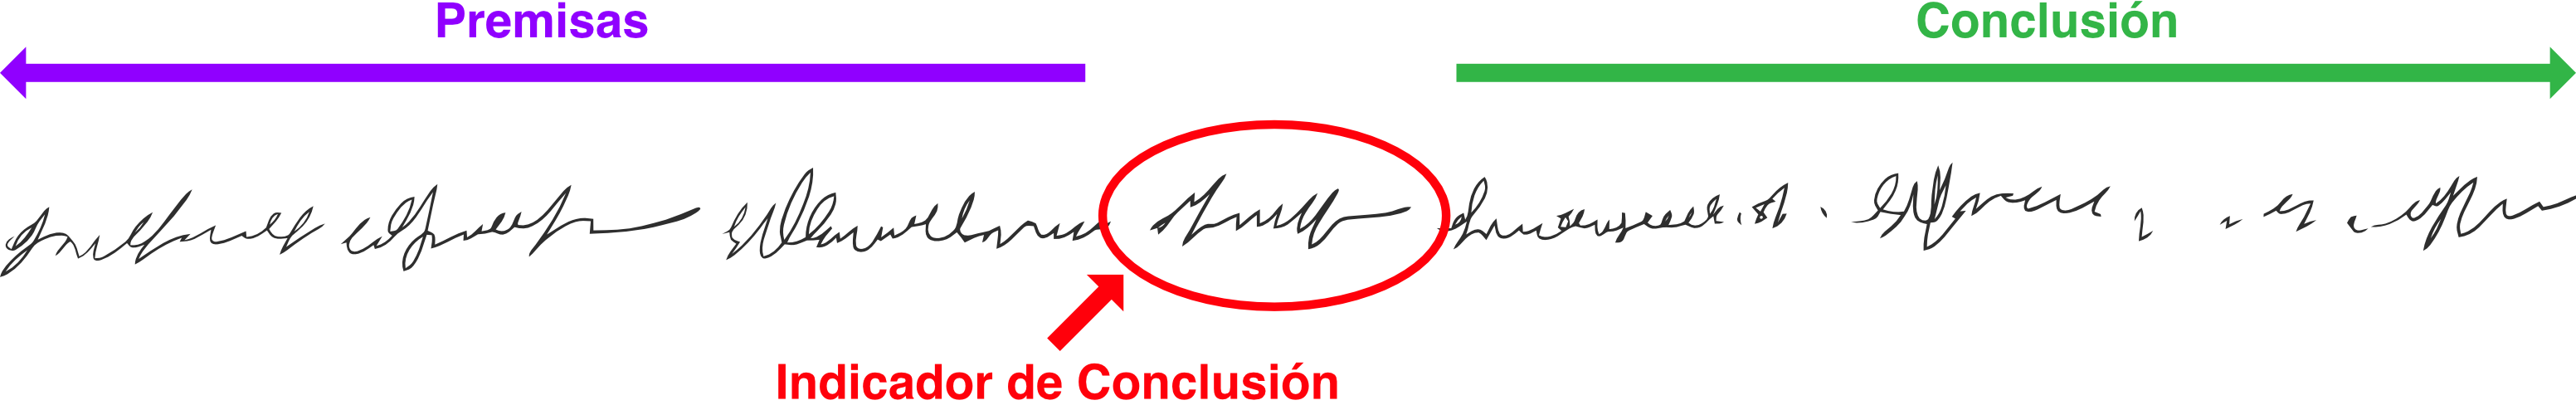
\includegraphics[scale=0.5]{unidades/3_logica/2_logica_proposicional/imagenes/indicadores_conclusion.png}

\subsection{Idicadores de premisa:}

También existen varias palabras que pueden actuar como indicadores de premisa. A
continuación se presenta una breve lista de estos.

\begin{minipage}{0.45\textwidth}
    \begin{itemize}
        \item Dado que
        \item Ya que
        \item Esto es así porque
        \item Porque
    \end{itemize}
\end{minipage}
\begin{minipage}{0.45\textwidth}
    \begin{itemize}
        \item Esto se sigue de
        \item En vista de que
        \item Pues
    \end{itemize}
\end{minipage}

Acá la idea es la inversa, es decir, que hay cosas que se cumplieron ya que
otras se habían cumplido antes, o de que algo ocurrió debído a que otras cosas
ocurrieron.

Con esto ya tenemos una idea más clara de cómo los razonamientos son
interpretados por la lógica proposicional, aunque los razonamientos que podemos
procesar son acotados, porque de momento conocemos solo tres conectivas.

En la sección siguiente veremos otra serie de conectivas que nos ayudarán a
plantear más y mejores razonamientos, y a posteriori veremos como los
razonamientos pueden ser analizados para determinar su validez.

Recordemos que un indicador de premisa separa las premisas de la conclusión de
forma tal que las premisas estarán \textbf{antes}, y la conclusión estará
\textbf{después}, del indicador, como se presenta en el siguiente gráfico:

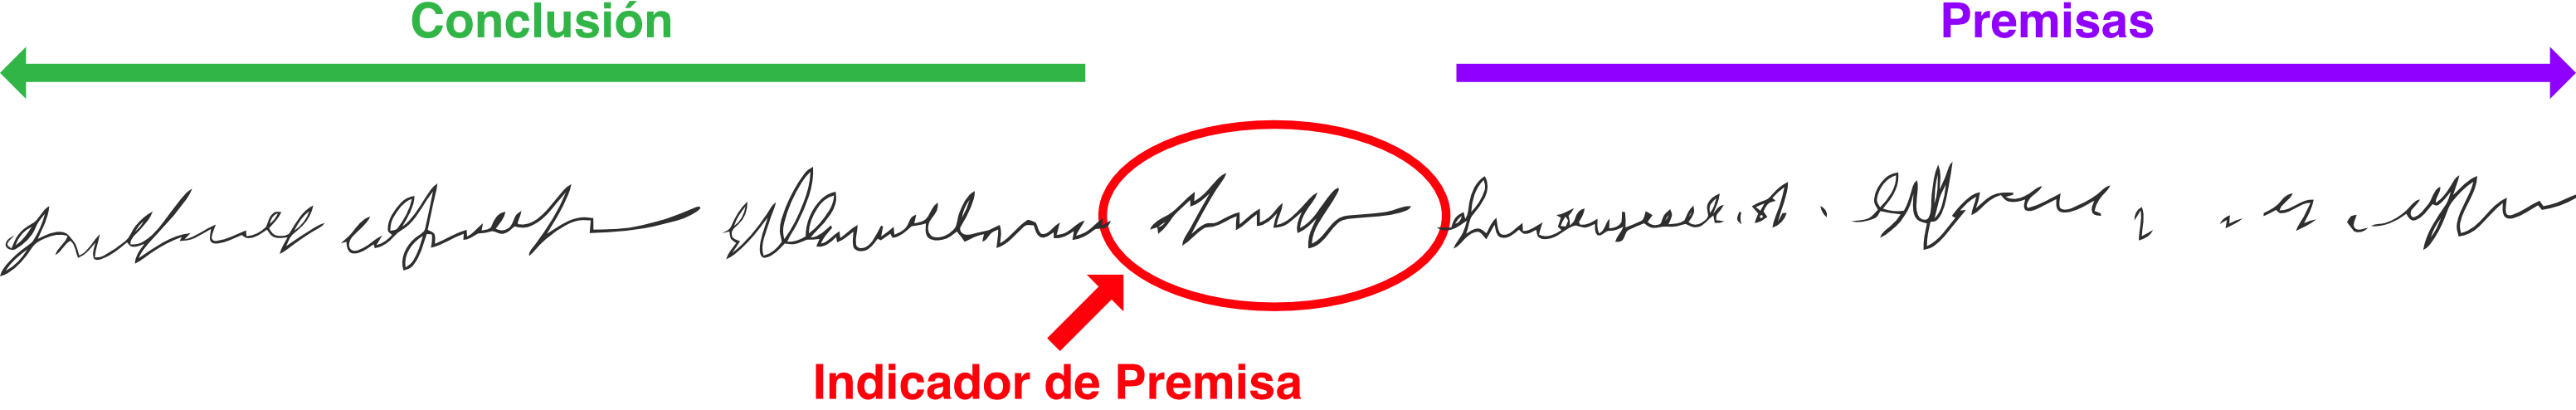
\includegraphics[scale=0.5]{unidades/3_logica/2_logica_proposicional/imagenes/indicadores_premisa.png}

Adicionalmente, y para finalizar esta sección, podemos mencionar que pueden
existir razonamientos en donde hay tanto indicadores de premisas como de
conclusión. En este caso, puede darse que la conclusión se encuentre en el medio
del razonamiento. El siguiente gráfico muestra esta idea.

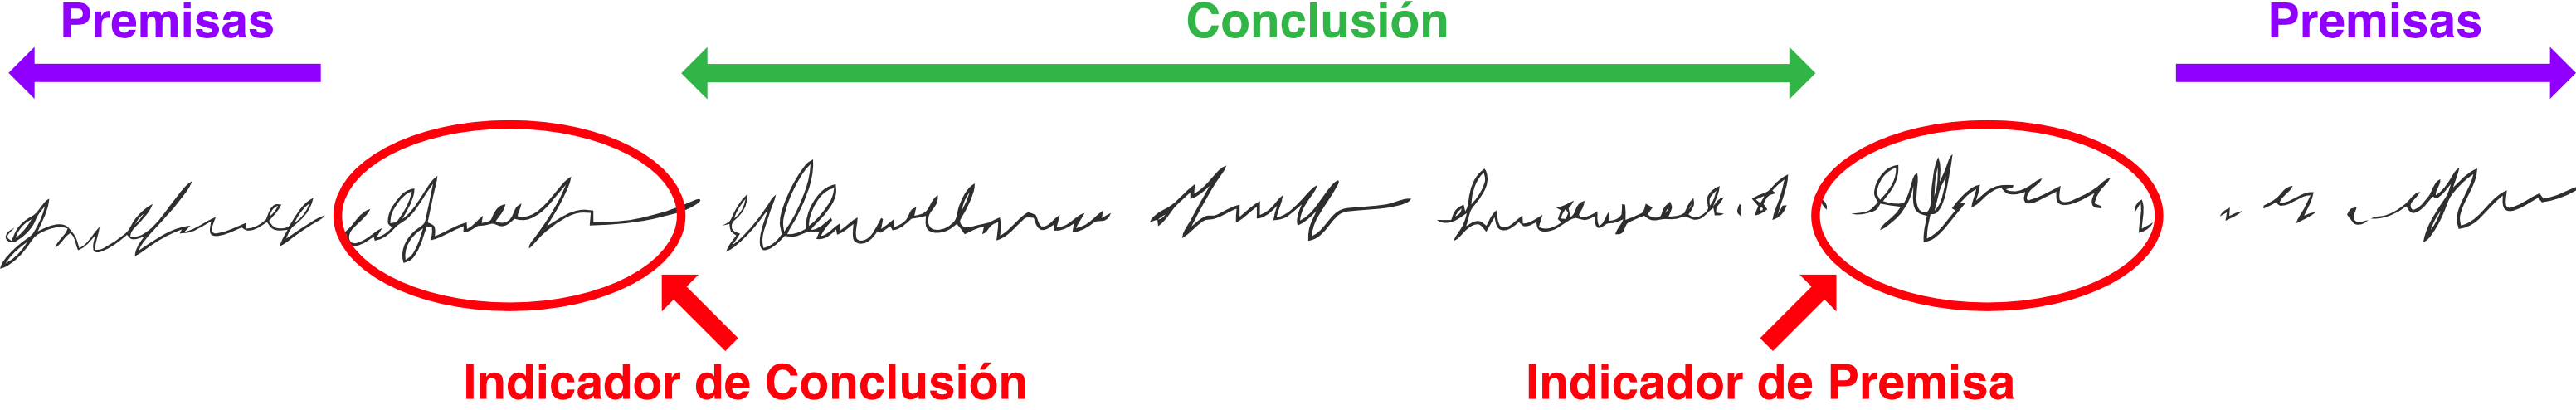
\includegraphics[scale=0.5]{unidades/3_logica/2_logica_proposicional/imagenes/indicadores_conclusion_y_premisa.png}

\section{Otras conectivas más complejas}
\label{chap:logica_proposicional:sec:otras_conectivas}

Hasta ahora hemos trabajado únicamente con tres conectivas, la conjunción, la
disyunción y la negación, que son las más comunes de encontrar en el lenguaje
natural en el habla cotidiana. Sin embargo, hay varias expresiones semánticas de
lenguajes naturales que no pueden expresarse con dichas conectivas, y que son
claves para poder escribir razonamientos interesantes.

En esta sección veremos entonces otra serie de conectivas que podemos hallar en
el lenguaje natural, su simbología, ejemplos y su tabla semántica.

\subsection{Disyunción excluyente}
\label{chap:logica_proposicional:subsec:xor}

Si pensamos en frases como ``\textit{El ascensor está detenido en un piso o bien
está moviendose}'' tal vez se nos ocurra representar esto mediante una
disyunción, algo como ``\textit{El ascensor está detenido en un piso $\lor$ El
ascensor está moviendose}''. Sin embargo, si consideramos que el ascensor no
puede estar en dos lugares al mismo tiempo, entonces ese ``\textit{o bien}'' no
nos habla de una disyunción normal, sino de una en donde puede ocurrir lo
primero o lo segundo, pero seguro no pueden suceder ambas cosas al mismo tiempo.

La idea de la \textbf{disyunción excluyente} es precisamente esa, la idea de
``\textbf{uno u otro, pero no ambos}''. En las proposiciones es posible
encontrar expresiones como ``\textit{Esta noche iré al cine o al teatro, pero no
a ambos}'', aunque no es tan común. Muchas veces, como en el ejemplo del
ascensor, simplemente encontraremos una palabra que refiere a la idea de
disyunción, y es el lector quien debe interpretar ambas partes y comprender que
no pueden suceder ambas al mismo tiempo.

Esto vuelve a veces dificil comprender en qué puntos hay disyunciones y en
cuales disyunciones excluyentes, en especial a quienes recién comienzan a
trabajar la idea de formalizar proposiciones enunciadas en el lenguaje natural.
Es importante entonces tomarnos un pequeño tiempo adicional para pensar si las
proposiciones unidas por la disyunción son excluyentes o no.

El símbolo que utilizamos para esta conectiva es $\lxor$, y su tabla semántica
es la siguiente:

\begin{tabular}{ c | c | c }
    \textbf{$\Phi$} & \textbf{$\Psi$} & \textbf{$\Phi \lxor \Psi$}\\
    \hline
    $\ltrue$  & $\ltrue$  & $\lfalse$ \\
    $\ltrue$  & $\lfalse$ & $\ltrue$  \\
    $\lfalse$ & $\ltrue$  & $\ltrue$  \\
    $\lfalse$ & $\lfalse$ & $\lfalse$ \\
\end{tabular}

Es decir, la disyunción excluyente indica que una expresión es verdadera solo
cuando se cumple una de las dos partes que la componen, pero no cuando se
cumplen ambas.

\subsection{Implicación}
\label{chap:logica_proposicional:subsec:then}

La \textbf{implicación} (también llamada \textbf{condicional}) es la conectiva
que se utiliza para la idea que una condición sucede solo si otra a sucedido. Es
decir, la idea de secuencia lógica, de que una cosa sucede de otra, en
consecuencia de la primera. Un ejemplo simple sería ``\textit{Si hay fuego,
entonces habrá humo}''. Es decir, el hecho de que haya humo es una consecuencia
de que haya fuego.

En términos semánticos, esta frase se debe considerar verdadera cuando, si
contrastamos con la realidad, efecivamente hay fuego y hay humo, lo cual sería
esperable, y falso si hubiera fuego pero no ocurre que haya humo. Si no hay
fuego, y no hay humo tampoco, entonces la frase también debe considerarse
verdadera. El caso que suele confundir a la mayoría es que la frase debe ser
considerada verdadera aún cuando no hay fuego, pero efectivamente hay humo. Si
lo pensamos, la frase habla de lo que ocurrirá cuando haya fuego, pero no dice
nada de lo que sucede si no hay fuego. Así, puede ser que no haya fuego y aún
así exista humo, producto de otra cosa, por ejemplo, una reacción quimica puede
producir humo sin que haya fuego involucrado.

El símbolo usado para la implicación es $\lthen$ y su tabla semántica sigue lo
recién mencionado:

\begin{tabular}{ c | c | c }
    \textbf{$\Phi$} & \textbf{$\Psi$} & \textbf{$\Phi \lthen \Psi$}\\
    \hline
    $\ltrue$  & $\ltrue$  & $\ltrue$  \\
    $\ltrue$  & $\lfalse$ & $\lfalse$ \\
    $\lfalse$ & $\ltrue$  & $\ltrue$  \\
    $\lfalse$ & $\lfalse$ & $\ltrue$  \\
\end{tabular}

Notar que la idea de implicación está muy relacionada a la idea de razonamiento,
ya que el indicador de conclusión también tiene una idea de secuencia. De hecho,
veremos que esta conectiva y esos indicadores de conclusión están intimamente
relacionados. Por supuesto, el problema surge al intentar identificar conectivas
en un razonamiento, donde las palabras que se utilizan para la conectiva de
implicación son similares a las que se utilizan como indicador de conclusión.
Algo a tener en cuenta es que el indicador de conclusión va a estar siempre al
comienzo de una oración (la cual es la conclusión) mientras que las conectivas
suelen estar a la mitad de una oración.

\subsection{Equivalencia}
\label{chap:logica_proposicional:subsec:iff}

La última conectiva que analizaremos será la conectiva de \textbf{equivalencia}
(también llamada \textbf{doble implicación} o \textbf{bicondicional}). Esta
conectiva deriva de la idea de ``\textbf{si y solo si}'', es decir, que algo
ocurre solo cuando otra cosa ocurre al mismo tiempo, y no ocurre solo cuando la
otra tampoco ocurre. Un ejemplo podría ser ``\textit{Ganaremos el torneo si y
solo si ganamos el próximo partido}''. Es decir, no puede darse que se gane el
torneo si no se gana el siguiente partido, y su inversa también se cumple, no se
ganará el torneo si no se gana el partido, algo que se da, por ejemplo, en una
final.

La semántica tiene además la idea de igualdad en términos lógicos, por ejemplo,
la frase ``\textit{Sentir la brisa y correr por el campo es lo mismo que correr
por el campo y sentir la brisa}'', lo cual habla de la idea de conmutatividad en
la lógica.

El símbolo de esta conectiva es $\liff$ y su tabla semántica es la siguiente:

\begin{tabular}{ c | c | c }
    \textbf{$\Phi$} & \textbf{$\Psi$} & \textbf{$\Phi \liff \Psi$}\\
    \hline
    $\ltrue$  & $\ltrue$  & $\ltrue$  \\
    $\ltrue$  & $\lfalse$ & $\lfalse$ \\
    $\lfalse$ & $\ltrue$  & $\lfalse$ \\
    $\lfalse$ & $\lfalse$ & $\ltrue$  \\
\end{tabular}

Este tipo de conectivas se utiliza mucho al momento de realizar demostraciones
matemáticas, y se vuelve de vital importancia en la misma. Por ejemplo, en $3 +
x = 7 \liff x = 4$.

\section{Formulas bien formadas}
\label{chap:logica_proposicional:sec:fbf}

Ahora que ya conocemos todas las conectivas, podemos hablar de cuándo una
fórmula de la lógica proposicional está \textbf{bien formada}. Una formula puede
no tener sentido, incluso si se usan los símbolos de las conectivas que hemos
visto. Por ejemplo, en matemática, si escribimos algo como \textit{$+5(\cdot
9($} nos encontramos ante símbolos matemáticos, pero sin sentido alguno. En la
lógica pasa lo mismo, las conectivas deben usarse de forma adecuada para que una
fórmula tenga sentido.

Toda variable proposicional es una \textbf{fórmula bien formada} (FBF). Es
decir, $p$, $q$, $r$, etc. son todas fórmulas bien formadas. Teniendo eso en
consideración, y suponiendo que $\Phi$ y $\Psi$ son fórmulas bien formadas,
todas las siguientes son también fórmulas bien formadas.
\begin{itemize}
    \item $(\lnot \Phi)$
    \item $(\Phi \land \Psi)$
    \item $(\Phi \lor \Psi)$
    \item $(\Phi \lxor \Psi)$
    \item $(\Phi \lthen \Psi)$
    \item $(\Phi \liff \Psi)$
\end{itemize}

Notar como todas las fórmulas mencionadas se encuentran entre paréntesis, ya que
esto será importante en un momento.

Pensemos ahora un ejemplo puntual. Queremos saber si la siguiente es una fórmula
bien formada o no. Para ello, debemos analizar desde adentro hacia afuera para
ver si se sumplen las reglas de formación de fórmulas bien formadas.

\begin{tabular}{l l l}
    & $((p \land (q \lor (\lnot r))) \land (r \lor p))$ & Se quiere probar si
    esta fórmula es una FBF.\\
    \hline
    1. & $p$ & Es una FBF por ser solo una variable proposicional\\
    2. & $q$ & Es una FBF por ser solo una variable proposicional\\
    3. & $r$  & Es una FBF por ser solo una variable proposicional\\
    4. & $(r \lor q)$ & Los paréntesis externos corresponden a una disyunción \\
    &&                  por lo que tanto $r$ como $q$ deben ser FBFs. 4. es\\
    &&                  entonces FBF ya que 2. y 3. prueban ser FBFs\\
    5. & $(\lnot r)$ &  Los paréntesis externos se corresponden a una
    negación,\\
    &&                  por lo que $r$ debe ser una FBF, y esto se prueba por
    3.\\
    6. & $(q \lor (\lnot r))$  & Los paréntesis externos corresponden a una
    disyunción,\\
    &&                           por lo que tanto $q$ como $(\lnot r)$ deben ser
    FBFs.\\
    &&                           Esto se prueba por 2. y por 5.\\
    7. & $(p \land (q \lor (\lnot r)))$ & Los paréntesis externos vuelven a
    corresponder a\\
    &&                           una conjunción, por lo que tanto $p$ como $(q
    \lor (\lnot r)$\\
    &&                           deben ser FBFs. Esto se prueba por 1. y por
    6.\\
    8. & $((p \land (q \lor (\lnot r))) \land (r \lor p))$ & Los paréntesis más
    externos corresponden a una conjunción,\\
    &&por lo que para este sea una FBF, tanto\\
    && $(p \land (q \lor (\lnot r))$ como $(r \lor p)$ deben ser FBFs.\\
    && Esto se prueba por 7. y por 4.
\end{tabular}

Los errores más comúnes al momento de escribir fórmulas que hacen que la fórmula
no esté bien formada suelen estar relacionadas a los siguientes ejemplos:

\begin{align}
    (p \lnot q) \tag*{Usar la negación como operador binario, en lugar de operador unario.}\\
    (\land p) \tag*{Usar un operador binario como un operador unario.}\\
    (p \land \lor q) \tag*{Usar dos operadores binarios de forma consecutiva}\\
    (p q) \tag*{Ausencia de operador entre dos variables proposicionales o fórmulas}\\
    (p (\land q)) \tag*{Aperturas o cierres de paréntesis en lugares incorrectos}\\
\end{align}


Así, es importante prestar especial atención para no cometer estos errores, y
asegurar que la fórmula que estamos escribiendo es una fórmula bien formada.

Sin embargo, cuando empezamos a analizar, los paréntesis de una fórmula bien
formada evitarán cualquier ambiguedad en la forma en la que debe interpretarse
la misma, pero la gran cantidad de los mismos resulta molesta. Para evitar
escribir algunos de ellos, vamos a seguir las siguientes reglas:

\begin{itemize}
    \item Los paréntesis más externos se omiten, siempre. Ej. la FBF \textit{$(p
    \land (q \lor r))$} podemos escribirla como \textit{$p \land (q \lor r)$}.
    \item La negación no llevará paréntesis externos. Ej. la FBF \textit{$(p
    \land (\lnot (q \land p)))$} podemos escribirla como \textit{$p \land \lnot
    (q \land p)$}.
    \item Varias ocurrencias del mismo operador no llevan paréntesis. Ej. Ej. la
    FBF \textit{$(p \land (q \land r))$} podemos escribirla como \textit{$p
    \land q \land r$} y la FBF \textit{$(\lnot (\lnot p))$} se puede escribir
    como \textit{$\lnot \lnot p$}.
    \item Podemos omitir paréntesis en todo lugar donde la precedencia deje en
    claro que operación debe analizarse primero que otra. Ej. la FBF
    \textit{$(((p \land q)) \lthen r)$} se puede escribir como \textit{$p \land
    q \lthen r$}
\end{itemize}

El hecho de omitir paréntesis no hace que la fórmula deje de ser bien formada,
sino que simplifica la complejidad de lectura de la misma. Ante la duda, es
preferible contar con los paréntesis, pero en este libro omitiremos aquellos que
no sean necesarios, salvo que los paréntesis ayuden a explicar un concepto o
tema.

\subsection{Orden de precedencia}
\label{chap:logica_proposicional:subsec:orden_precedencia }

El \textbf{orden de precedencia} tiene que ver con la prioridad con la que
leemos determinados símbolos en una fórmula. Ya habíamos visto la misma en la
\autoref{chap:logica:sec:precedencia}, pero ahora debemos definir una nueva
precedencia, ya que hay nuevos símbolos. La precedencia que usaremos será:

\begin{enumerate}
    \item Negación
    \item Conjunción
    \item Disyunción
    \item Implicación
    \item Equivalencia
\end{enumerate}

Es decir, que la negación asocia más fuerte, luego la conjunción, la disyunción,
la implicación, y por último la equivalencia. Esto permite eliminar paréntesis,
ya que los elementos que asocian más fuerte no necesitan paréntesis para indicar
que su interpretación debe ser previa a otros elementos. Así \textit{$(((()\lnot
p) \land q)) \lthen r)$} se puede escribir como \textit{$\lnot p \land q \lthen
r$} ya que la precedencia nos permite simplificar los paréntesis.

\section{Analisis de validez de razonamientos por tabla de verdad}
\label{chap:logica_proposicional:sec:validez }

Ahora que sabemos como detectar un razonamiento e identificar sus partes, vamos
a querer poder determinar si el mismo es \textbf{válido} o no. Pero, ¿Qué
significa que un razonamiento sea válido?

\begin{definition}
    Un razonamiento se dice \textbf{válido}\index{Valido@Válido} cuando
    \textbf{las premisas implican a la conclusión}. Es decir, que si sus
    premisas son verdaderas, entonces la conclusión es necesariamente verdadera.
\end{definition}

Es decir, lo que tiene que ocurrir es que si para cada valuación donde todas las
premisas son verdaderas, entonces la conclusión en cada una de esas valuaciones
también debe ser verdadera.

Analicemos el razonamiento a continuación para poder comprender la idea. Vamos a
    realizar el pasaje a fórmula del razonamiento junto con la presentación del
    mismo, pero el lector puede intentar realizar paso a paso la identificación
    de las partes como se presentó en la sección anterior\footnote{ Recuerde que
    al momento de armar el diccionario debe reformular las proposiciones para
    simplificar elementos gramaticales y los tiempos verbales. }.

\begin{example}
    \sindent Razonamiento en lenguaje natural:

    \dindent Si hay fuego entonces habrá humo. Pero no hay humo. Por lo tanto,
    no había fuego.

    \sindent Diccionario:

    \dindent $f = \text{Hay fuego}$

    \dindent $h = \text{Hay humo}$

    \sindent Fórmula:

    \dindent $f \lthen h, \lnot h \lseq f$
\end{example}

Vamos a elaborar ahora la tabla de verdad para este razonamiento. Para un
razonamiento, a diferencia de para una símple proposición, donde nos interesa
llegar a una única columna final, aquí debemos asegurarnos de tener una columna
para cada premisa, y una columna para la conclusión. Por supuesto, puede que sea
necesario elaborar columnas intermedias para resolver los diversos pasos, antes
de arribar a alguna de las columnas que nos interesan, algo que ocurrirá cuando
la fórmula sea compleja .

Comenzaremos entonces por elaborar una tabla donde ``$f$'' y ``$h$'' (las
variables proposicionales) son los elementos base. En nuestro ejemplo, no
necesitaremos columnas intermedias, ya que las fórmulas tienen todas una única
conectiva, por lo que iremos directamente a colocar una columna para cada
premisa, y una para la conclusión.

\centerline{
\begin{tabular}{ c | c | c | c | c }
     &  & Premisa 1 & Premisa 2 & Conclusión \\
    $f$ & $h$ & $f \lthen h$ & $\lnot h$ & $\lnot f$\\
    \hline
    $\ltrue$  & $\ltrue$  & & &  \\
    $\ltrue$  & $\lfalse$ & & &  \\
    $\lfalse$ & $\ltrue$  & & &  \\
    $\lfalse$ & $\lfalse$ & & &
\end{tabular}
}

Como ya dijimos, al no haber pasos intermedios, mirando $f$ y $h$ podemos
completar todas las columnas restantes.

\centerline{
\begin{tabular}{ c | c | c | c | c }
    &  & Premisa 1 & Premisa 2 & Conclusión \\
    $f$ & $h$ & $f \lthen h$ & $\lnot h$ & $\lnot f$\\
    \hline
    $\ltrue$  & $\ltrue$  & $\ltrue$  & $\lfalse$ & $\lfalse$ \\
    $\ltrue$  & $\lfalse$ & $\lfalse$ & $\ltrue$  & $\lfalse$ \\
    $\lfalse$ & $\ltrue$  & $\ltrue$  & $\lfalse$ & $\ltrue$ \\
    $\lfalse$ & $\lfalse$ & $\ltrue$  & $\ltrue$  & $\ltrue$
\end{tabular}
}

Ahora que tenemos la tabla lista, cabe preguntarse si este razonamiento es
válido o no. Lo que nos va a interesar no son las proposiciones atómicas, sino
solamente las premisas y la conclusión, por lo que eliminaremos las dos primeras
columnas.

\centerline{
\begin{tabular}{ c | c | c }
    Premisa 1 & Premisa 2 & Conclusión \\
    $f \lthen h$ & $\lnot h$ & $\lnot f$\\
    \hline
    $\ltrue$  & $\lfalse$ & $\lfalse$ \\
    $\lfalse$ & $\ltrue$  & $\lfalse$ \\
    $\ltrue$  & $\lfalse$ & $\ltrue$  \\
    $\ltrue$  & $\ltrue$  & $\ltrue$
\end{tabular}
}

Ahora bien, debemos tener presente lo que significa que el razonamiento sea
válido. Cuando un razonamiento es válido, para todos los casos en donde la
totalidad de las premisas sea verdadera, la conclusión debe también ser
verdadera. Busquemos primero las filas donde las premisas son ambas verdaderas.

\centerline{
\begin{tabular}{ c | c | c }
    Premisa 1 & Premisa 2 & Conclusión \\
    $f \lthen h$ & $\lnot h$ & $\lnot f$\\
    \hline
    $\ltrue$  & $\lfalse$ & $\lfalse$ \\
    $\lfalse$ & $\ltrue$  & $\lfalse$ \\
    $\ltrue$  & $\lfalse$ & $\ltrue$  \\
    \cellcolor{yellow}$\ltrue$  & \cellcolor{yellow}$\ltrue$  & $\ltrue$
\end{tabular}
}

Como vemos, esto se cumple únicamente en la última fila (hemos marcado con
amarillo las premisas en ese caso para que sea fácil de identificar). Una vez
identificada las filas que cumplen el criterio, debemos verificar que para cada
una de ellas, la conclusión sea también verdadera. En este caso, podemos ver que
también lo es.

\centerline{
\begin{tabular}{ c | c | c }
    Premisa 1 & Premisa 2 & Conclusión \\
    $f \lthen h$ & $\lnot h$ & $\lnot f$\\
    \hline
    $\ltrue$  & $\lfalse$ & $\lfalse$ \\
    $\lfalse$ & $\ltrue$  & $\lfalse$ \\
    $\ltrue$  & $\lfalse$ & $\ltrue$  \\
    \cellcolor{yellow}$\ltrue$  & \cellcolor{yellow}$\ltrue$  &
    \cellcolor{cyan}$\ltrue$
\end{tabular}
}

Así, decimos que el razonamiento es \textbf{válido}. En el caso de que para
cualquiera de las filas en donde las premisas son verdaderas la conclusión sea
falsa, el razonamiento será \textbf{inválido}.

Veamos un segundo ejemplo, un poco más complejo. Esta vez iremos directamente
por la fórmula de un razonamiento, sin importar cuál es el razonamiento concreto
del cual se obtuvo.

\begin{example}
    \sindent $(p \lthen q) \lthen r, \lnot p \lseq r$
\end{example}

En este caso hay solo dos premisas, ya no tan simple la primera de ellas, por lo
que necesitaremos pasos intermedios para calcular su valor de verdad en cada
valuación de la tabla. La conclusión es trivial nuevamente. Realizaremos la
tabla de verdad de manera idéntica a como lo hicimos en las ocasiones previas.

\centerline{
\begin{tabular}{ c | c | c | c | c | c  }
    & & Conclusión & & Premisa 1 & Premisa 2 \\
    $p$ & $q$ & $r$ & $p \lthen q$ & $(p \lthen q) \lthen r$ & $\lnot p$\\
    \hline
    $\ltrue$  & $\ltrue$  & $\ltrue$  & $\ltrue$  & $\ltrue$ & $\lfalse$ \\
    $\ltrue$  & $\ltrue$  & $\lfalse$ & $\ltrue$  & $\lfalse$ & $\lfalse$ \\
    $\ltrue$  & $\lfalse$ & $\ltrue$  & $\lfalse$ & $\ltrue$  & $\lfalse$ \\
    $\ltrue$  & $\lfalse$ & $\lfalse$ & $\lfalse$ & $\ltrue$  & $\lfalse$ \\
    $\lfalse$ & $\ltrue$  & $\ltrue$  & $\ltrue$  & $\ltrue$ & $\ltrue$ \\
    $\lfalse$ & $\ltrue$  & $\lfalse$ & $\ltrue$  & $\lfalse$ & $\ltrue$ \\
    $\lfalse$ & $\lfalse$ & $\ltrue$  & $\ltrue$  & $\ltrue$ & $\ltrue$ \\
    $\lfalse$ & $\lfalse$ & $\lfalse$ & $\ltrue$  & $\lfalse$ & $\ltrue$
\end{tabular}
}

Podemos apreciar que la conclusión termina coincidiendo con una de las variables
proposicionales, motivo por el cual aparece antes que las premisas. Primero,
eliminemos todos los pasos intermedios, que fueron solo necesarios para calcular
el valor de las premisas y conclusión, y quitemos también las variables
proposicionales (no $r$, pues es la conclusión). Como el orden de las columnas
no es importante, aprovecharemos además para cambiar el orden de los elementos,
dejando la conclusión al final, para un análisis posterior más sencillo.

\centerline{
\begin{tabular}{ c | c | c }
    Premisa 1 & Premisa 2 & Conclusión \\
    $(p \lthen q) \lthen r$ & $\lnot p$ & $r$ \\
    \hline
    $\ltrue$  & $\lfalse$ & $\ltrue$  \\
    $\lfalse$ & $\lfalse$ & $\lfalse$ \\
    $\ltrue$  & $\lfalse$ & $\ltrue$  \\
    $\ltrue$  & $\lfalse$ & $\lfalse$ \\
    $\ltrue$  & $\ltrue$  & $\ltrue$  \\
    $\lfalse$ & $\ltrue$  & $\lfalse$ \\
    $\ltrue$  & $\ltrue$  & $\ltrue$  \\
    $\lfalse$ & $\ltrue$  & $\lfalse$
\end{tabular}
}

Buscaremos los lugares donde ámbas premisas sean verdaderas.

\centerline{
\begin{tabular}{ c | c | c }
    Premisa 1 & Premisa 2 & Conclusión \\
    $(p \lthen q) \lthen r$ & $\lnot p \land q$ & $r$ \\
    \hline
    $\ltrue$  & $\lfalse$ & $\ltrue$  \\
    $\lfalse$ & $\lfalse$ & $\lfalse$ \\
    $\ltrue$  & $\lfalse$ & $\ltrue$  \\
    $\ltrue$  & $\lfalse$ & $\lfalse$ \\
    \cellcolor{yellow} $\ltrue$  & \cellcolor{yellow} $\ltrue$  & $\ltrue$  \\
    $\lfalse$ & $\ltrue$  & $\lfalse$ \\
    \cellcolor{yellow} $\ltrue$  & \cellcolor{yellow} $\ltrue$ & $\ltrue$  \\
    $\lfalse$ & $\ltrue$ & $\lfalse$
\end{tabular}
}

Como vemos hay dos valuaciones en donde las premisas son verdaderas al mismo
tiempo. Es decir, lo que nos interesa es que en cada una de esas filas la
conclusión sea verdadera.

\centerline{
\begin{tabular}{ c | c | c }
    Premisa 1 & Premisa 2 & Conclusión \\
    $(p \lthen q) \lthen r$ & $\lnot p \land q$ & $r$ \\
    \hline
    $\ltrue$  & $\lfalse$ & $\ltrue$  \\
    $\lfalse$ & $\lfalse$ & $\lfalse$ \\
    $\ltrue$  & $\lfalse$ & $\ltrue$  \\
    $\ltrue$  & $\lfalse$ & $\lfalse$ \\
    \cellcolor{yellow} $\ltrue$  & \cellcolor{yellow} $\ltrue$  &
    \cellcolor{cyan}$\ltrue$  \\
    $\lfalse$ & $\ltrue$  & $\lfalse$ \\
    \cellcolor{yellow} $\ltrue$  & \cellcolor{yellow} $\ltrue$ &
    \cellcolor{cyan} $\ltrue$  \\
    $\lfalse$ & $\lfalse$ & $\lfalse$
\end{tabular}
}

En este caso, vemos que efectivamente ocurre que la conclusión es verdadera
cuando las premisas lo son, por lo que el razonamiento termina por ser válido.

Trabajaremos un último ejemplo. Este es similar al anterior, pero una de las
premisas ha sido cambiada.

\begin{example}
    \sindent $(p \lthen q) \lthen r, p \lseq r$
\end{example}

Siendo qye ya hemos visto en reiteradas ocasiones como realizar la tabla de
verdad paso a paso, iremos directo a la tabla final de este razonamiento.

\centerline{
\begin{tabular}{ c | c | c }
    Premisa 1 & Premisa 2 & Conclusión \\
    $(p \lthen q) \lthen r$ & $p$ & $r$ \\
    \hline
    $\ltrue$  & $\ltrue$ & $\ltrue$  \\
    $\lfalse$ & $\ltrue$ & $\lfalse$ \\
    $\ltrue$  & $\ltrue$ & $\ltrue$  \\
    $\ltrue$  & $\ltrue$ & $\lfalse$ \\
    $\ltrue$  & $\lfalse$ & $\ltrue$  \\
    $\lfalse$ & $\lfalse$ & $\lfalse$ \\
    $\ltrue$  & $\lfalse$ & $\ltrue$  \\
    $\lfalse$ & $\lfalse$ & $\lfalse$
\end{tabular}
}

Nuevamente, para que el razonamiento sea válido, tenemos que buscar los lugares
donde las premisas sean todas verdaderas, y verificar que allí la conclusión
también lo sea.

\centerline{
\begin{tabular}{ c | c | c }
    Premisa 1 & Premisa 2 & Conclusión \\
    $(p \lthen q) \lthen r$ & $p$ & $r$ \\
    \hline
    \cellcolor{yellow} $\ltrue$  & \cellcolor{yellow} $\ltrue$ &\cellcolor{cyan}
    $\ltrue$  \\
    $\lfalse$ & $\ltrue$ & $\lfalse$ \\
    \cellcolor{yellow} $\ltrue$  & \cellcolor{yellow} $\ltrue$ &
    \cellcolor{cyan} $\ltrue$  \\
    \cellcolor{yellow} $\ltrue$  & \cellcolor{yellow} $\ltrue$ &
    \cellcolor{cyan} $\lfalse$ \\
    $\ltrue$  & $\lfalse$ & $\ltrue$  \\
    $\lfalse$ & $\lfalse$ & $\lfalse$ \\
    $\ltrue$  & $\lfalse$ & $\ltrue$  \\
    $\lfalse$ & $\lfalse$ & $\lfalse$
\end{tabular}
}

Podemos apreciar como en la tercer fila, valuación que tiene a $p$ por
verdadero, $q$ por falso, y $r$ por verdadero, da como resultado premisas
verdaderas, pero una conclusión falsa. Es esta fila la que nos indica que el
razonamiento es \textbf{inválido}, ya que encontramos un caso en donde, ante
premisas verdaderas, la conclusión termina por ser falsa, violando lo que
plantean los razonamientos deductivos.

\section{Relación entre las premisas y la conclusión}
\label{chap:logica_proposicional:sec:relacion_premisas_conclusion}

Hemos mencionado como, en un razonamiento proposicional, cuando las premisas so
verdaderas, la conclusión debe ser necesariamente verdadera. Otra forma de
plantear esto es decir que ``\textbf{Las premisas implican lógicamente a la
conclusión}''.

Esto quiere decir que hay una relación lógica entre las premisas y la conclusión
que sigue la siguiente forma:

\begin{corollary}
    $\text{premisa 1} \land \text{premisa 2} \land \ldots land \text{premisa N}
    \lthen \text{conclusión}$
\end{corollary}

Detengamonos un segundo uno de los razonamientos ya analizados, ``\textit{El
gato en la caja está o bien vivo o bien muerto. Pero el gato no estaba muerto.
Por lo tanto, el gato estaba vivo.}''. El indicador de conclusión, en el
lenguaje natural, coincide en gran medida con las palabras que indican una
implicación en una proposición compuesta. Esto se debe a que efectivamente
expresa una idea de implicación, entre las premisas y la conclusión. Más aún,
ese ``\textit{Pero}'' que en su momento habíamos dejado de lado, coincide con
una palabra que se usa para conjunción. Esto es así porque efectivamente cumple
el rol de conjunción entre las premisas.

Si nos detenemos sobre la fórmula de dicho razonamiento, ``$p \lor \lnot p,
\lnot \lnot p \lseq p$'', podemos ver que es posible probar el razonamiento
mediante su tabla de verdad y analisis posterior, de la siguiente forma:

\centerline{
\begin{tabular}{ c | c | c }
    Premisa 1 & Premisa 2 & Conclusión \\
    $p \lor \lnot p$ & $\lnot \lnot p$ & $p$\\
    \hline
    \cellcolor{yellow}$\ltrue$  & \cellcolor{yellow}$\ltrue$ & \cellcolor{cyan}
    $\ltrue$  \\
    $\ltrue$ & $\lfalse$ & $\lfalse$ \\
\end{tabular}
}

Otra forma para probar que el razonamiento sea válido sería calcular que las
premisas impliquen a la conlcusión, es decir, que ``$(p \lor \lnot p) \land
(\lnot \lnot p) \lthen p$'' sea una \textbf{tautología}. Recordemos que, que sea
tautología significa que siempre es verdadera, para cualquier valuación.

\centerline{
\begin{tabular}{ c | c | c | c }
    Premisa 1 & Premisa 2 & Conclusión & Prueba de razonamiento completo \\
    $p \lor \lnot p$ & $\lnot \lnot p$ & $p$ &  $(p \lor \lnot p) \land ()\lnot
    \lnot p)\lthen p$\\
    \hline
    $\ltrue$  &$\ltrue$ & $\ltrue$  &  \cellcolor{cyan} $\ltrue$\\
    $\ltrue$ & $\lfalse$ & $\lfalse$ &  \cellcolor{cyan} $\ltrue$\\
\end{tabular}
}

Esto prueba el razonamiento, porque quiere decir que solo en aquellos casos
donde las premisas sean verdaderas, la concusión también debe serlo, pero nada
importa si las premisas son falsas.

Si nos detenemos a pensar la semántica de un razonamiento es donde podemos
comprender la idea completa de lo que estamos hablando. Salgamos de las tablas
de verdad y vayamos a un ejemplo sencillo ``\textit{Si yo soy Superman, entonces
puedo volar. Y resulta que efectivamente soy Superman. Por lo tanto, es cierto
que puedo volar.}''. Con ese razonamiento en mente, subo a un noveno piso
vestido con una capa roja, y salto desde el balcón\ldots Por supuesto, la caída
va a ser fatal.

El problema no está en el razonamiento en sí, el cual tiene una estructura
perfectamente válida\footnote{Puede el lector realizar el pasaje a fórmular y
analizar la tabla de verdad del mismo como ejercicio.}, sino en las premisas. Si
contrastamos con la realidad, sabemos que Superman es un personaje de ficción,
que no existe, y que cualquier afirmación sobre que alguien sea Superman es
falsa. \textbf{Partir de premisas falsas lleva a conclusiones incorrectas,
incluso ante un razonamiento perfectamente válido}. La lógica no se ocupa sobre
la realidad de las premisas en contraste con la realidad, sino sobre el analisis
del razonamiento en si, y queda en quien enuncia el razonamiento, asegurarse que
las premisas tengan sentido.

Podemos entonces concluir que en un razonamiento hay una relación (lógica) entre
premisas y conclusión. Esa relación está dada por la forma del razonamiento, y
no por el contenido del mismo. Sin embargo, aunque la lógica estudia la relación
dada por la forma, no analiza en ningun momento el contenido, el cual deberá ser
sometido a contrastaciones empíricas si fuera necesario.

\section{Álgebra de Boole}
\label{chap:logica_proposicional:sec:algebra_boole}

En 1857 George Boole publicó ``\textit{An investigation of the Laws of Tought}''
(Una investigación sobre las Leyes del Pensamiento), una obra que postula
procesos de análisis sobre elementos lógicos, con una completa explicación sobre
los procesos de inferencia y deducción. La publicación es considerada como una
obra fundacional, ya que establece procesos matemáticos (formales) para trabajar
con la lógica, algo novedoso para la época.

A posteriori de su obra, otros autores ampliaron los conocimientos sobre la
lógica, se formalizaron y descubrieron teoremas, nuevas formas de análisis, etc.
elaborando un completo sistema formal al que se suele llamar \textbf{Álgebra de
Boole}.

Los principios básicos de este álgebra versan sobre lo ya charlado en esta
unidad, valores de verdad, proposiciones y conectivas, y análisis lógico de los
valores de verdad expresados en proposiciones compuestas o razonamientos. Sin
embargo, el álgebra de Boole equematiza las operaciones lógicas, permitiendo
establecer teoremas y realizar pruebas sobre las fórmulas.

No vamos a meternos en la definición del álgebra de Boole, que es compleja y
requiere un buen entendimiento matemático, sino más bien en los corolarios que
de esta surgen, y como estos aplican a la lógica proposicional, por lo que esta
sección será solo un vistazo simple a esta parte de la lógica.

\subsection{Equivalencia de fórmulas}
\label{chap:logica_proposicional:subsec:equivalencia_boole}

Decimos que dos fórmulas son equivalentes cuando, ante una misma valuación, se
obtiene el mismo resultado en ambas formulas, y esto ocurre para toda valuación.

\begin{definition}
    Dos fórmulas se dicen \textbf{equivalentes} cuando producen el mismo valor
    de verdad ante una misma valuación, para toda valuación posible.
\end{definition}

Un ejemplo podrían ser las fórmulas $p \land q$ y la fórmula $q \land p$.
Equivalencia que podemos probar por tabla de verdad.

\centerline{
\begin{tabular}{ c | c | c | c }
    $p$ & $q$ & $p \land q$ & $q \land p$\\
    \hline
    $\ltrue$  & $\ltrue$  & $\ltrue$  & $\ltrue$ \\
    $\ltrue$  & $\lfalse$ & $\lfalse$ & $\lfalse$ \\
    $\lfalse$ & $\ltrue$  & $\lfalse$ & $\lfalse$ \\
    $\lfalse$ & $\lfalse$ & $\lfalse$ & $\lfalse$ \\
\end{tabular}
}

Si analizamos las últimas dos columnas, vemos como los valores que resultan son
idénticos, en cada fila de la tabla. Esto nos habla de la equivalencia, la cual
también puede probarse verficando que dos fórmulas unidas con una conectiva de
equivalencia producen una tautología. En este ejemplo, verificar que $(p \land
q) \liff (q \land p)$ produce efectivamente una tautología.

\centerline{
\begin{tabular}{ c | c | c | c | c }
    $p$ & $q$ & $p \land q$ & $q \land p$ & $(p \land q) \liff (q \land p)$ \\
    \hline
    $\ltrue$  & $\ltrue$  & $\ltrue$  & $\ltrue$  & $\ltrue$ \\
    $\ltrue$  & $\lfalse$ & $\lfalse$ & $\lfalse$ & $\ltrue$ \\
    $\lfalse$ & $\ltrue$  & $\lfalse$ & $\lfalse$ & $\ltrue$ \\
    $\lfalse$ & $\lfalse$ & $\lfalse$ & $\lfalse$ & $\ltrue$ \\
\end{tabular}
}

De hecho, lo que acabamos de probar no es otra cosa que la \textbf{propiedad
conmutativa} en la conjunción.

El álgebra de Boole se basa en este tipo de equivalencias para establecer sus
\textbf{axiomas}, es decir, caracteristicas que debe cumplir un sistema formal
para ser un álgebra de Boole, en donde se definen relaciones entre las
operaciones lógicas y los valores de verdad, y desde donde surgen los
\textbf{teoremas}, postulados formales que surgen de los axiomas o de otros
teoremas ya probados.

\subsection{Axiomas y Leyes del Álgebra de Boole}
\label{chap:logica_proposicional:subsec:leyes_algebra_boole}

El álgebra de Boole presenta 10 axiomas (5 en dos sabores diferentes), que son
los siguientes.

{\noindent\raggedleft
\begin{minipage}{0.45\textwidth}
    \begin{enumerate}[label=\arabic*a]
        \item Ley de \textbf{identidad} en la cojunción\\
            $\Phi \land \ltrue \liff \Phi$
        \item Existencia del \textbf{elemento complementario} en la cojunción\\
            $\Phi \land \lnot \Phi \liff \lfalse$
        \item Ley \textbf{asociativa} de la conjunción\\
            $(\Phi \land \Psi) \land \Tau \liff \Phi \land (\Psi \land \Tau)$
        \item Ley \textbf{conmutativa} de la conjunción\\
            $\Phi \land \Psi \liff \Psi \land \Phi$
        \item Ley \textbf{distributiva} de la conjunción respecto a la
        disyunción\\
            $\Phi \land (\Psi \lor \Tau) \liff (\Phi \land \Psi) \lor (\Phi
            \land \Tau)$
    \end{enumerate}
\end{minipage}
\begin{minipage}{0.45\textwidth}
    \begin{enumerate}[label=\arabic*b]
        \item Ley de \textbf{identidad} en la disyunción\\
            $\Phi \lor \lfalse \liff \Phi$
        \item Existencia del \textbf{elemento complementario} en la disyunción\\
            $\Phi \lor \lnot \Phi \liff \ltrue$
        \item Ley \textbf{asociativa} de la disyunción\\
            $(\Phi \lor \Psi) \lor \Tau \liff \Phi \lor (\Psi \lor \Tau)$
        \item Ley \textbf{conmutativa} de la disyunción\\
            $\Phi \lor \Psi \liff \Psi \lor \Phi$
        \item Ley \textbf{distributiva} de la disyunción respecto a la
        conjunción\\
            $\Phi \lor (\Psi \land \Tau) \liff (\Phi \lor \Psi) \land (\Phi \lor
            \Tau)$
    \end{enumerate}
\end{minipage}
}

Partiendo de los axiomas anteriores se pueden probar algunas leyes
fundamentales.

{\noindent\raggedleft
\begin{minipage}{1\textwidth}
    \begin{enumerate}[label=\arabic*a, start=6]
        \item Ley de \textbf{involución}\\
            $\lnot (\lnot \Phi) \liff \Phi$
    \end{enumerate}
\end{minipage}
}

{\noindent\raggedleft
\begin{minipage}{0.45\textwidth}
    \begin{enumerate}[label=\arabic*a, start=7]
        \item Ley de \textbf{idempotencia} en la conjunción\\
            $\Phi \land \Phi \liff \Phi$
        \item Ley de \textbf{absorción} en la conjunción\\
            $\Phi \land \lfalse \liff \lfalse$
        \item Ley de \textbf{De Morgan} (para la conjunción)\\
            $\lnot (\Phi \land \Psi) \liff \lnot \Phi \lor \lnot \Psi$
        \item Ley de \textbf{complemento} (caso 1)\\
            $\lnot \ltrue \liff \lfalse$
    \end{enumerate}
\end{minipage}
\begin{minipage}{0.45\textwidth}
    \begin{enumerate}[label=\arabic*a, start=7]
        \item Ley de \textbf{idempotencia} en la conjunción\\
            $\Phi \lor \Phi \liff \Phi$
        \item Ley de \textbf{absorción} en la conjunción\\
            $\Phi \lor \ltrue \liff \ltrue$
        \item Ley de \textbf{De Morgan} (para la disyunción)\\
            $\lnot (\Phi \lor \Psi) \liff \lnot \Phi \land \lnot \Psi$
        \item Ley de \textbf{complemento} (caso 2)\\
            $\lnot \lfalse \liff \ltrue$
    \end{enumerate}
\end{minipage}
}

\begin{knowwhat}
    El álgebra de Boole tiene una definición mucho más formal, y aplica no solo
    a la lógica proposicional, sino a la matemática binaria o la teoría de
    conjuntos. Cada rama emplea una notación distinta para referirse a los
    mismos elementos, por ejemplo, el lógica digital se suelen emplear los
    signos \textit{0} y \textit{1} para lo que nosotros estamos mencionando como
    $\lfalse$ y $\ltrue$, y en conjuntos usan a idea de $\varnothing$ y de $U$.
    También cambian los signos que se usan para los operaciones.
\end{knowwhat}

La aplicación sucesiva de estas leyes permite solucionar o simplificar fórmulas
lógicas, como se muestra a continuación:

\begin{example}
\begin{align}
\lnot p \land (\lnot (\lnot p \land q)) \tag*{(Aplicando De Morgan)}\\
\lnot p \land ((\lnot \lnot p) \lor (\lnot q))) \tag*{(Aplicando distributiva)}\\
(\lnot p \land (\lnot \lnot p)) \lor (\lnot p \land \lnot q) \tag*{(Aplicando involución)}\\
(\lnot p \land p) \lor (\lnot p \land \lnot q) \tag*{(Aplicando elemento complementario)}\\
\lfalse \lor (\lnot p \land \lnot q) \tag*{(Aplicando conmutativa)}\\
(\lnot p \land \lnot q) \lor \lfalse \tag*{(Aplicando identidad)}\\
\lnot p \land \lnot q \tag*{(Aplicando De Morgan, invertida)}\\
\lnot (p \lor q)
\end{align}
\end{example}

\section{Reglas de inferencia}
\label{chap:logica_proposicional:sec:inferencia}

Cuando Aristóteles comenzó a analizar la lógica y formalizarla, desarrolló
también las \textbf{reglas de inferencia}. En su concepción más simple, podemos
decir que una regla de inferencia es un razonamiento de estructura bien conocida
a la que se le da un nombre particular. Su definición formal, sin embargo, es la
de una función que permite obtener una conclusión dada una serie de premisas.

\begin{definition}
    Una \textbf{regla de inferencia}, o también \textbf{regla de transformación}
    es una función que toma premisas como entrada, analiza su sintaxis y
    describe una conclusión como salida.
\end{definition}

Es decir, si tenemos una serie de premisas que cumplen una estructura
particular, que cae dentro de uno de los casos de inferencia, podemos determinar
fácilmente su conclusión. Por supuesto, las reglas de inferencia pueden
combinarse entre si, y con las reglas de reemplazo del álgebra de Boole, para
obtener conclusiones más complejas.

A continuación veremos  algunas de las reglas que fueron determinadas por
Aristóteles en la antiguedad, y que es bueno tener en consideración a la hora de
pensar razonamientos. Por supuesto no son las únicas reglas existentes, pero
trabajaremos sobre otras en las actividades finales de este capítulo.

\subsection{Modus ponendo ponens}

El \textit{\textbf{modus ponendo ponens}}, latin para \textbf{el modo que, al
afirmar, afirma}, también llamado \textbf{afirmación del antecedente} es una
regla con la siguiente forma:

\begin{minipage}{0.3\textwidth}
    \begin{lreasoning}
        \lpremise{$\Phi \lthen \Psi$}
        \lpremise{$\Phi$}
        \lconclusion{$\Psi$}
    \end{lreasoning}
\end{minipage}

Podemos analizar fácilmente este razonamiento. Si el antecedente es verdadero,
la única forma de que la implicación sea verdadera es que el consecuente sea
también verdadero. Así, si sabemos que vale la implicación, y que vale el
antecedente, podemos concluir que necesariamente debe valer el concecuente.

Un ejemplo de este tipo de razonamientos es el siguiente:

\begin{minipage}{0.5\textwidth}
    \begin{lreasoning}
        \lpremise{Si hay fuego, entonces habrá humo}
        \lpremise{Hay fuego}
        \lconclusion{Hay humo}
    \end{lreasoning}
\end{minipage}

Podríamos analizar por tabla de verdad este razonamiento, verificando su
validez, aunque esto se deja como ejercicio para el lector.

\subsection{Modus tollendo tollens}

El \textit{\textbf{modus tollendo tollens}}, latin para \textbf{el modo que, al
negar, niega}, también llamado \textbf{negación del consecuente} es una regla
con la siguiente forma:

\begin{minipage}{0.3\textwidth}
    \begin{lreasoning}
        \lpremise{$\Phi \lthen \Psi$}
        \lpremise{$\lnot \Psi$}
        \lconclusion{$\lnot \Phi$}
    \end{lreasoning}
\end{minipage}

Podemos nuevamente analizar fácilmente que este razonamiento es válido. Si
sabemos que el consecuente es falso, pero la implicación es verdadera, entonces
no hay forma alguna de que el antecedente sea verdadero, pues si lo fuera la
implicación sería falsa. Solo puede darse entonces como conclusión que el
antecedente es necesariamente falso.

Si seguimos la misma implicación del ejemplo anterior, el razonamiento sería:

\begin{minipage}{0.5\textwidth}
    \begin{lreasoning}
        \lpremise{Si hay fuego, entonces habrá humo}
        \lpremise{No hay humo}
        \lconclusion{No hay fuego}
    \end{lreasoning}
\end{minipage}

Es importante destacar que la premisa es la negación del consecuente, y no del
antecedente, ya que de la negación de este último no podría elaborarse ninguna
conclusión, algo que analizamos en la
\autoref{chap:logica_proposicional:sec:falacias}.

\subsection{Modus ponendo tollens}

El \textit{\textbf{modus ponendo tollens}}, latin para \textbf{el modo que, al
afirmar, niega}, es una regla que establece que, si no es posible que dos
proposiciones sean verdaderas al mismo tiempo, y una de ellas es verdadera,
entonces la otra debe ser necesariamente falsa. La fórmula de este razonamiento
es:

\begin{minipage}{0.3\textwidth}
    \begin{lreasoning}
        \lpremise{$\lnot (\Phi \land \Psi)$}
        \lpremise{$\Phi$}
        \lconclusion{$\lnot \Psi$}
    \end{lreasoning}
\end{minipage}

Un ejemplo en lenguaje natural podría ser el siguiente:

\begin{minipage}{0.5\textwidth}
    \begin{lreasoning}
        \lpremise{No es cierto que Gómez y Rodriguez puedan ser ámbos presidentes al mismo tiempo}
        \lpremise{Gómez es presidente}
        \lconclusion{No es cierto que Rodriguez sea presidente}
    \end{lreasoning}
\end{minipage}

Nuevamente el análisis es sencillo. La única forma de que la conjunción sea
verdadera, es cuando ámbas proposiciones son verdaderas. La negación antes de la
conjunción es verdadera siempre, salvo en el caso de la conjunción verdadera (Es
decir, afirma que no pueden ocurrir $\Phi$ y $\Psi$ al mismo tiempo). El hecho
de que ocurra uno de ellos, hace obligatorio que el otro no ocurra para que la
premisa sea verdadera, y por tanto la única conclusión posible es que la otra
proposición debe ser falsa.

\subsection{Modus tollendo ponens}

El \textit{\textbf{modus tollendo ponens}}, latin para \textbf{el modo que, al
negar, afirma}, es una regla que establece que, si una de dos proposiciones debe
ser verdadera, y una de ellas es falsa, entonces la otra debe ser necesariamente
verdadera. La fórmula de este razonamiento es:

\begin{minipage}{0.3\textwidth}
    \begin{lreasoning}
        \lpremise{$\Phi \lor \Psi$}
        \lpremise{$\lnot \Phi$}
        \lconclusion{$\Psi$}
    \end{lreasoning}
\end{minipage}

Para que la disyunción sea verdadera, uno de los elementos debe ser verdadero.
Si sabemos que uno de ellos es falso (por la segunda premisa), entonces podemos
concluir que la otra proposición es verdadera.

Un ejemplo en lenguaje natural podría ser el siguiente:

\begin{minipage}{0.5\textwidth}
    \begin{lreasoning}
        \lpremise{O bien Gomez es presidente o bien Rodriguez es presidente}
        \lpremise{Gómez no es presidente}
        \lconclusion{Rodriguez es entonces el presidente}
    \end{lreasoning}
\end{minipage}

Todas estas reglas de inferencia nos permiten entender mejor las conectivas y
los razonamientos, y entender de mejor forma cuándo un razonamiento es válido y
cuándo no. Si bien podemos siempre probar un razonamiento mediante tablas de
verdad, la realidad es que si nos encontramos con un razonamiento que sigue una
de las reglas de inferencia, podríamos simplemente afirmar su validez, ya que la
misma fue probada hace más de 2000 años.

\section{Falacias bien conocidas}
\label{chap:logica_proposicional:sec:falacias}

Así como hay formas bien conocidas de razonamientos válidos, también hay formas
bien conocidas de razonamientos inválidos, llamados \textbf{falacias}. Las
falacias tienen estructuras que, para el ojo no entrenado, resultan válidas,
pero que realmente no lo son.

Conocer las falacias nos permite entender mejor las estructuras de los
razonamientos válidos, pero también los inválidos. Conocerlas nos evita caer en
errores comunes. Veremos entonces algunas de las falacias más comunes que
podemos encontrar.

\subsection{Afirmación del consecuente}

La \textit{\textbf{afirmación del consecuente}} es tal vez uno de los errores
más comunes. Su estructura es la siguiente:

\begin{minipage}{0.3\textwidth}
    \begin{lreasoning}
        \lpremise{$\Phi \lthen \Psi$}
        \lpremise{$\Psi$}
        \lconclusion{$\Phi$}
    \end{lreasoning}
\end{minipage}

Es decir, sabiendo verdadera la implicación, y verdadero su consecuente, se
afirma que vale el antecedente. Un ejemplo en lenguaje natural sería:

\begin{minipage}{0.5\textwidth}
    \begin{lreasoning}
        \lpremise{Si hay fuego, entonces habrá humo}
        \lpremise{Hay humo}
        \lconclusion{Hay fuego}
    \end{lreasoning}
\end{minipage}

Se puede ver en la tabla de verdad, si analizamos las valuaciones donde las
premisas son verdaderas, que la conclusión no necesariamente lo es en toda
valuación:

\centerline{
\begin{tabular}{ c | c | c }
    Premisa 1 & Premisa 2 & Conclusión \\
    $\Phi \lthen \Psi$ & $\Psi$ & $\Phi$ \\
    \hline
    \cellcolor{yellow}$\ltrue$  & \cellcolor{yellow}$\ltrue$  &
    \cellcolor{yellow}$\ltrue$  \\
    $\lfalse$ & $\lfalse$ & $\ltrue$  \\
    \cellcolor{yellow}$\ltrue$  & \cellcolor{yellow}$\ltrue$  &
    \cellcolor{yellow}$\lfalse$ \\
    $\ltrue$  & $\lfalse$ & $\lfalse$ \\
\end{tabular}
}

De hecho ya hemos analizado anteriormente este caso, el humo en realidad podría
haberse producido por otros motivos, que no son la presencia de fuego. La
implicación solo dice que sucede cuando el antecedente se cumple, no cuando no
se cumple, y el consecuente podría ser verdadero incluso con el antecedente
falso, y la implicación seguiría siendo verdadera.

\subsection{Negación del antecedente}

La implicación suele ser lo que más dolores de cabeza trae a los recién
iniciados, y por eso la \textbf{negación del antecedente} es otra forma de
falacia bien conocida, cuya fórmula para el razonamiento es:

\begin{minipage}{0.3\textwidth}
    \begin{lreasoning}
        \lpremise{$\Phi \lthen \Psi$}
        \lpremise{$\lnot \Phi$}
        \lconclusion{$\lnot \Psi$}
    \end{lreasoning}
\end{minipage}

Surge de la confusión de que, si sucede el antecedente entonces sucederá el
consecuente, y por tanto afirmar su inversa (si no sucede el antecedente
entonces tampoco sucederá el consecuente). Como vimos, esto no es cierto,
incluso si el antecedente es falso, el consecuente podría ser perfectamente
verdadero, manteniendo verdadera a la implicación. Un ejemplo sería

\begin{minipage}{0.5\textwidth}
    \begin{lreasoning}
        \lpremise{Si hay fuego, entonces habrá humo}
        \lpremise{No hay fuego}
        \lconclusion{No hay humo}
    \end{lreasoning}
\end{minipage}

Nuevamente, ya hemos discutido como el humo puede producirse por otros motivos
que no sean la presencia de fuego.

\section{Límites de la lógica proposicional}
\label{chap:logica_proposicional:sec:limites}

Vamos a volver sobre nuestros pasos para formalizar un razonamiento que ya hemos
visto.

\begin{example}
    \textit{Todos los humanos son mortales. Sócrates es un humano. Por lo tanto, Socrates es mortal.}
\end{example}

En primer lugar, podemos identificar que ``\textit{Por lo tanto}'' es el
indicador de conclusión. Esto hace que ``\textit{Socrates es mortal}'' sea la
conclusión, mientras que las otras dos oraciones sean las premisas.

Si intentamos pasar todo a fórmula veremos que se requieren tres variables
proposicionales, ya que las tres oraciones afirman cosas diferentes. Es decir,
el diccionario y la fórmula resultantes serían:

\begin{example}
    \sindent Diccionario:

    \dindent $p$ = Todos los humanos son mortales.

    \dindent $q$ = Sócrates es humano.

    \dindent $r$ = Sócrates es mortal.

    \sindent Fórmula:

    \begin{lreasoning}[width=0.6\textwidth,margin=\value{dindentwidth} pt]
        \lpremise{$p$}
        \lpremise{$q$}
        \lconclusion{$r$}
    \end{lreasoning}
\end{example}

Inmediatamente podemos apreciar que este razonamiento es falso, pues la
conclusión es algo completamente independiente de las premisas, y estas no son
contradictorias.

\begin{knowwhat}
    En los razonamientos deductivos la conclusión siempre se desprende de las
    premisas. Es decir, tras el pasaje a fórmula siempre la conclusión debe
    incluir proposiciones que estén mencionadas en las premisas, aunque estás
    pueden estar combinadas de formas diferentes a como lo estaban en las
    premisas.

    La única situación en donde la conclusión puede no desprenderse de las
    premisas es la reducción al absurdo, es decir, cuando las premisas se
    prueban necesariamente falsas y absurdar. Un ejemplo es afirmar que vale $p$
    y al mismo tiempo vale $\lnot p$ en las premisas. Por ser una situación
    imposible, cualquier conclusión que surja de dichas premisas es válida,
    incluso si nada tiene que ver con las premisas.
\end{knowwhat}

Sin embargo, cuando leemos el razonamiento, nos resulta intuitivo pensar en su
validez. ¿Es acaso realmente inválido? Bueno, si, lo acabamo de analizar. Pero,
¿Dónde está el truco? Si vemos la estructura interna vamos a apreciar que, si
bien no aparece dos veces la misma proposición, si hay elementos que se repiten
internamente entre las distintas proposiciones.

\begin{example}
    \begin{lreasoning}[width=0.6\textwidth,margin=\value{dindentwidth} pt]
        \lpremise{Todos los humanos son mortales}
        \lpremise{Sócrates es un humano}
        \lconclusion{Sócrates es mortal}
    \end{lreasoning}
\end{example}

Sócrates es siempre el mismo, tanto en la premisa como en la conclusión. La idea
de ``ser un humano'' o de ``ser mortal'' también aparece en más de una ocasión.
Sin embargo la lógica proposicional no permite reflejar esa estructura
gramatical.

El gran problema entonces es que este tipo de razonamientos caen fuera de lo que
la lógica proposicional permite modelar. Es decir, no se pueden formalizar
adecuadamente razonamientos en donde la semántica está relacionada a la
estructura gramatical interna de las proposiciones. Este tipo de razonamientos
no tiene solución en la lógica proposicional, hemos llegado al límite de la
misma.

Deberemos entonces recurrir a un nuevo formalismo para poder modelar este
razonamiento de forma apropiada. En el \autoref{chap:logica_predicados} se
propone otro sistema lógico, que permite solucionar el problema de este
razonamiento, pero también de otros.

\section{Actividades}
\label{chap:logica_proposicional:sec:actividades}

\begin{exercise}
    Identifique cuales de las siguientes son proposiciones y cuales no lo son.

    \begin{enumerate}[a]
        \item Microsoft es la empresa detrás del sistema operativo Windows.
        \item ¿Hay vida en Marte?
        \item Las células eucariotas tienen núcleo y las procariotas no lo
        tienen.
        \item ¡Bienvenidos chicos!
        \item ¿Es un celular inteligente?
        \item No es cierto que haya empresas que beneficien a algunos políticos.
        \item Las leyes más importantes.
    \end{enumerate}
\end{exercise}

\begin{exercise}
    Identifique las conectivas y las proposiciones atómicas involucradas, luego
    realice la traducción al lenguaje de la lógica proposicional de las
    siguientes oraciones:

    \begin{enumerate}[a]
      \item Safari es un navegador y viene instalado en macOS.
      \item Safari es un navegador o bien es un sistema operativo.
      \item Safari es un navegador, y no es cierto que viene instalado en
      Windows.
      \item O bien vamos al cine o bien al teatro, más no ambos, pero
      compraremos pochoclos.
      \item Linux puede funcionar en computadoras de escritorio, en dispositivos
      móviles o en otros dispositivos.
      \item GIMP no es ni un sistema operativo ni un navegador.
      \item Manjaro es una distribución de Linux basada en Arch y viene con el
          escritorio Gnome, el escritorio KDE y con otros escritorios populares.
      \item No es cierto que Debian sea la distribución más vieja de Linux, pero
        Slackware si lo es.
      \item El software son los programas y el SO de una PC, o bien, son los
      componentes físicos y periféricos de una PC.
      \item Solo encontraremos vida en marte si vamos a dicho planeta.
      \item Si viene Richard Stallman a la Argentina, iré a verlo y le pediré un
      autógrafo.
      \item Me encanta ver jugar a Messi ya que es un gran jugador de fútbol y a
      mi me gusta ese deporte.
      \item Argentina solo saldrá de su penosa situación económica si llega al
      poder un gobierno fuerte con ideas nuevas.
    \end{enumerate}
\end{exercise}

\begin{exercise}
    A partir de los siguiente enunciados, determine cuales son
    \textbf{proposiciones} solamente y cuales son \textbf{razonamientos}.

    En caso de que sean proposiciones diga además si es atómica o compuesta,
    encontrando las conectivas.

    En caso de ser un razonamiento, diga cuales son las premisas y cual la
    conclusión, identificando el indicador de premisa/conclusión que se esta
    utilizado.

    \begin{enumerate}[a]
        \item Empezaré karate y judo.
        \item O bien me inscribo a judo y a karate, o bien a jiu jitsu. Me
        inscribí en jiu jitsu. Por lo tanto, no me inscribí a karate y a judo.
        \item Voy a cursar los martes y los viernes. Ya que, o bien iba a cursar
        los lunes y jueves, o bien los martes y viernes. Pero no voy a cursar
        los lunes.
        \item Me inscribí a jiu jitsu.
        \item Si me inscribo a karate me volveré muy fuerte. Pero no me volví
        muy fuerte. Por lo tanto, no me inscribí a karate.
        \item No es cierto que uno se vuelva fuerte ya que se inscribió a jiu
        jitsu.
    \end{enumerate}
\end{exercise}

\begin{exercise}
    Determine cuáles de las siguientes son fórmulas bien formadas, y cuáles no
    lo son.

    \begin{enumerate}[a]
        \item $p \lthen q \land r$
        \item $p \lor q \lnot p$
        \item $p \land (\lnot q \liff \lnot r)$
        \item $p \land (\land q \lthen r)$
        \item $p \land (q (\lthen r))$
        \item $p \land \lnot q \liff \lnot r$
    \end{enumerate}
\end{exercise}

\begin{exercise}
    Analice los siguientes razonamientos y extrapole la fórmula lógica de cada
    proposición. Luego, pruebe si el razonamiento es válido o inválido.

    \begin{enumerate}[a]
        \item Si hay bananas o hay manzanas entonces hay fruta. No hay manzanas.
        Por tanto, no hay fruta.

        \item Si se comienza a tratar el calentamiento global se podrá detener a
        tiempo. Pero no se comienza a trata el calentamiento global. Por tanto,
        no se podrá detener a tiempo.

        \item No es cierto que se deba detener el ascensor. Dado que, el
        ascensor se debe detener si y solo si está frente a la puerta de un
        piso. Y no es cierto que el ascensor esté frente a la puerta de un piso.

        \item Se han movilizado tropas aliadas al norte. Por lo tanto, hay
        ejércitos enemigos al norte. Ya qué si no hay ejércitos enemigos al
        norte entonces no es necesario movilizar tropas aliadas en esa
        dirección.

        \item Si un software es libre, entonces tiene una licencia libre. Si un
        software tiene licencia libre entonces garantiza las cuatro libertades
        del software libre. Por lo tanto, si un software es libre, entonces
        garantiza las cuatro libertades del software libre.

        \item La teoría de cuerdas une la gravedad con la mecánica cuántica, por
        tanto, es una teoría de como funciona nuestro universo. La teoría de
        cuerdas requiere de diez dimensiones para funcionar. En consecuencia,
        nuestro universo cuenta con diez dimensiones.

        \item Hay que verificar su existencia o hay que tener fé ciega en su
        existencia. Es posible verificar su existencia si y solo si se cuenta
        con el equipo adecuado. No se cuenta con el equipo adecuado. En
        consiguiente, hay que tener fé ciega en su existencia.

        \item Si y solo si se cuenta con suficiente dinero se podrá construir el
        edificio. Si se ha vendido suficiente cantidad de mineral, entonces se
        contará con suficiente dinero. Por ende, se puede construir el edificio.

        \item Si cambia el panorama político de la AFA entonces la situación
        futbolística se revierte. Adicionalmente, el panorama político de la AFA
        no va a cambiar si el presidente de la AFA no toma una decisión radical
        o no sucede que alguien más accede a la dirección. Por consiguiente, si
        el presidente toma una decisión política radical o alguien más accede a
        la dirección es que cambiará el panorama político de la AFA.

        \item La Tierra es plana o es redonda. Si la Tierra es redonda entonces
        no nos caeremos por el borde. En cambio, si la Tierra es plana, si nos
        caeremos por el borde. Pero la Tierra no es plana. En consecuencia, no
        nos caeremos por el borde.

        \item El ascensor está en movimiento. Esto es así ya que si el ascensor
        no abre sus puertas es porque o bien está en movimiento, o bien se está
        preparando para moverse. Y la puerta está cerrada y el ascensor no se
        está preparando para moverse.

        \item Si la celda actual está pintada de rojo y la celda siguiente a la
        derecha está pintada de negro, entonces el cabezal se moverá dos lugares
        a la derecha. El cabezal no se movió dos lugares a la derecha. En
        consiguiente, o bien la celda actual no estaba pintada de rojo, o bien
        la celda siguiente a la derecha no estaba pintada de negro.

        \item Los pasajeros no murieron. Por tanto, la U.S.S Enterprise los
        transportó con éxito en la superficie. Ya qué, si la U.S.S. Enterprise
        no los transportaba con éxito en la superficie, entonces los pasajeros
        morirían.

    \end{enumerate}
\end{exercise}

\begin{exercise}
    Analice las siguientes implicaciones y determine en cada situación si
\end{exercise}

\begin{exercise}
    Dadas las siguientes estructuras lógicas formalizadas de razonamientos,
    analizar si los mismos son válidos o inválidos.

    \begin{enumerate}
        \item $p \land q \lseq p$
        \item $p \lxor q, \lnot q \lseq p$
        \item $p \lor q, \lnot q \lseq \lnot p$
        \item $p \lor q, \lnot q \lseq p$
        \item $p \lthen q, p \lseq q$
        \item $\lnot p \lthen q, \lnot q \lseq \lnot p$
        \item $p \lthen q, \lnot q \lseq \lnot p$
        \item $p \lthen q, q \lthen r, p \lseq r$
        \item $(p \lor q) \lthen r, p \land \lnot q \lseq r$
        \item $(p \lxor q) \lthen r, \lnot p \land \lnot q \lseq r$
    \end{enumerate}
\end{exercise}

TODO Ejercicio sobre probar el resto de las reglas de inferencia y/o falacias

\begin{exercise}
    A partir de las siguientes estructuras lógicas de razonamientos, piense
    distintas proposiciones en lenguaje natural o ejemplos que se pueden aplicar
    a los mismos:

    \begin{enumerate}
        \item
            \begin{lreasoning}[width=0.4\textwidth]
                \lpremise{$p \lxor q$}
                \lpremise{$\lnot q$}
                \lconclusion{$p$}
            \end{lreasoning}

        \item
            \begin{lreasoning}[width=0.4\textwidth]
                \lpremise{$p \lxor q$}
                \lpremise{$p$}
                \lconclusion{$\lnot q$}
            \end{lreasoning}

        \item
            \begin{lreasoning}[width=0.4\textwidth]
                \lpremise{$p \lthen q$}
                \lpremise{$p$}
                \lconclusion{$q$}
            \end{lreasoning}

        \item
            \begin{lreasoning}[width=0.4\textwidth]
                \lpremise{($p \land q) \lthen \lnot s$}
                \lpremise{$p \land q$}
                \lconclusion{$\lnot s$}
            \end{lreasoning}
     \end{enumerate}
\end{exercise}


\begin{exercise}
    Dados los siguientes razonamientos, identifique los indicadores de premisa,
    los indicadores de conclusión, y estructure el razonamiento en premisas y
    conclusión.

    \begin{enumerate}
        \item Si hay bananas o hay manzanas, entonces hay fruta. No hay
        manzanas. Pero hay fruta. Por lo tanto, hay bananas.

        \item Será Santino quien venga a la fiesta. Dado que a la fiesta iba a
        venir o bien Guadalupe o bien Santino. Pero Guadalupe no va a venir.

        \item Argentina clasificó para el mundial FIFA 2022. Esto es así porque
        o bien Perú clasifica para el mundial o bien Argentina clasifica para el
        mundial. Pero Perú no clasificó.

        \item Instagram es la red social más utilizada. Dado que Instagram es la
        red social más utilizada y Facebook se utiliza cada vez menos.

        \item Me compro un pantalón o me compro una remera, pero no ambas. Me
        compre una remera. Por lo tanto, me compre un pantalón o no me compre un
        pantalón.
      \end{enumerate}
    \end{exercise}

\begin{exercise}
    Determine si las siguientes expresiones son equivalentes. Para ello primero
    traduzca del lenguaje natural al lenguaje formal de la lógica proposicional,
    y utilice la conectiva correspondiente para unir ambas expresiones y
    comprobar si son equivalentes o no.

    \begin{enumerate}
      \item
        ¿Será lo mismo la frase \textbf{``Hay vida en Marte y hay vida en
        Ganimedes''} a la frase \textbf{``Hay vida en Ganimedes y hay vida en
        Marte''}?

      \item
        ¿Será lo mismo la frase \textbf{``Hay vida en Marte o hay vida en
        Ganimedes''} a la frase \textbf{``Hay vida en Ganimedes o hay vida en
        Marte''}?

      \item
        ¿Será lo mismo la frase \textbf{``Si hay vida en Marte entonces hay vida
        en Ganimedes''} a la frase \textbf{``Si hay vida en Ganimedes entonces
        hay vida en Marte''}?

      \item
        ¿Será lo mismo la frase \textbf{``No es cierto que no hay vida en
        Marte''} a la frase \textbf{``Hay vida en Marte''}?

      \item
        ¿Será lo mismo la frase \textbf{``No es cierto que, hay vida en Marte o
        hay vida en Ganimedes''} a la frase \textbf{``No hay vida en Marte y no
        hay vida en Ganimedes''}?


      \item
        ¿Será lo mismo la frase \textbf{``No es cierto que, hay vida en Marte y
        hay vida en Ganimedes''} a la frase \textbf{``No hay vida en Marte o no
        hay vida en Ganimedes''}?

    \end{enumerate}
\end{exercise}

\begin{exercise}
    Pruebe que los axiomas del álgebra de Boole se cumplen, verificando las
    equivalencias expresadas.
\end{exercise}
